\documentclass[11pt, a4paper]{book}
%\errorcontextlines 10000
\usepackage[utf8]{inputenc}
\usepackage[italian]{babel}
\usepackage[T1]{fontenc}

\usepackage{tabularx}
\usepackage[table]{xcolor}

% required to include the thesis first page
\usepackage{pdfpages}


% specifying lmodern as default font, uses it on the entire document
% (before doing this, It used different fonts along the document...)
\usepackage{lmodern}

% listing required for quote management
\usepackage{textcomp}

\usepackage{graphicx}
\usepackage{wrapfig}
\graphicspath{ {immagini/} }

\usepackage{mathtools}

\usepackage{listings}
\renewcommand{\lstlistingname}{Listato}
\renewcommand{\lstlistlistingname}{Elenco dei listati}
\lstset{upquote=true, breaklines=true, columns=flexible}
% Thanks to: https://tex.stackexchange.com/questions/64839/how-to-change-listing-caption

\usepackage[backend=biber]{biblatex}
\addbibresource{thesis_citations.bib}

\usepackage[justification=justified]{caption}
\usepackage{subcaption}

\usepackage[binary-units=true]{siunitx}

%TODO: source https://tex.stackexchange.com/questions/9796/how-to-add-todo-notes
\usepackage[colorinlistoftodos,prependcaption,textsize=tiny]{todonotes}

\newcommand{\addcontent}[1]{\todo[inline,linecolor=green,backgroundcolor=green!25,bordercolor=green,]{#1}}

\newcommand {\pygfa} {\textit{PyGFA}}

\title{\pygfa \\
	Progettazione ed implementazione di una libreria Python per la gestione
	di file GFA}
\author{Diego Lobba}

\begin{document}
% \maketitle
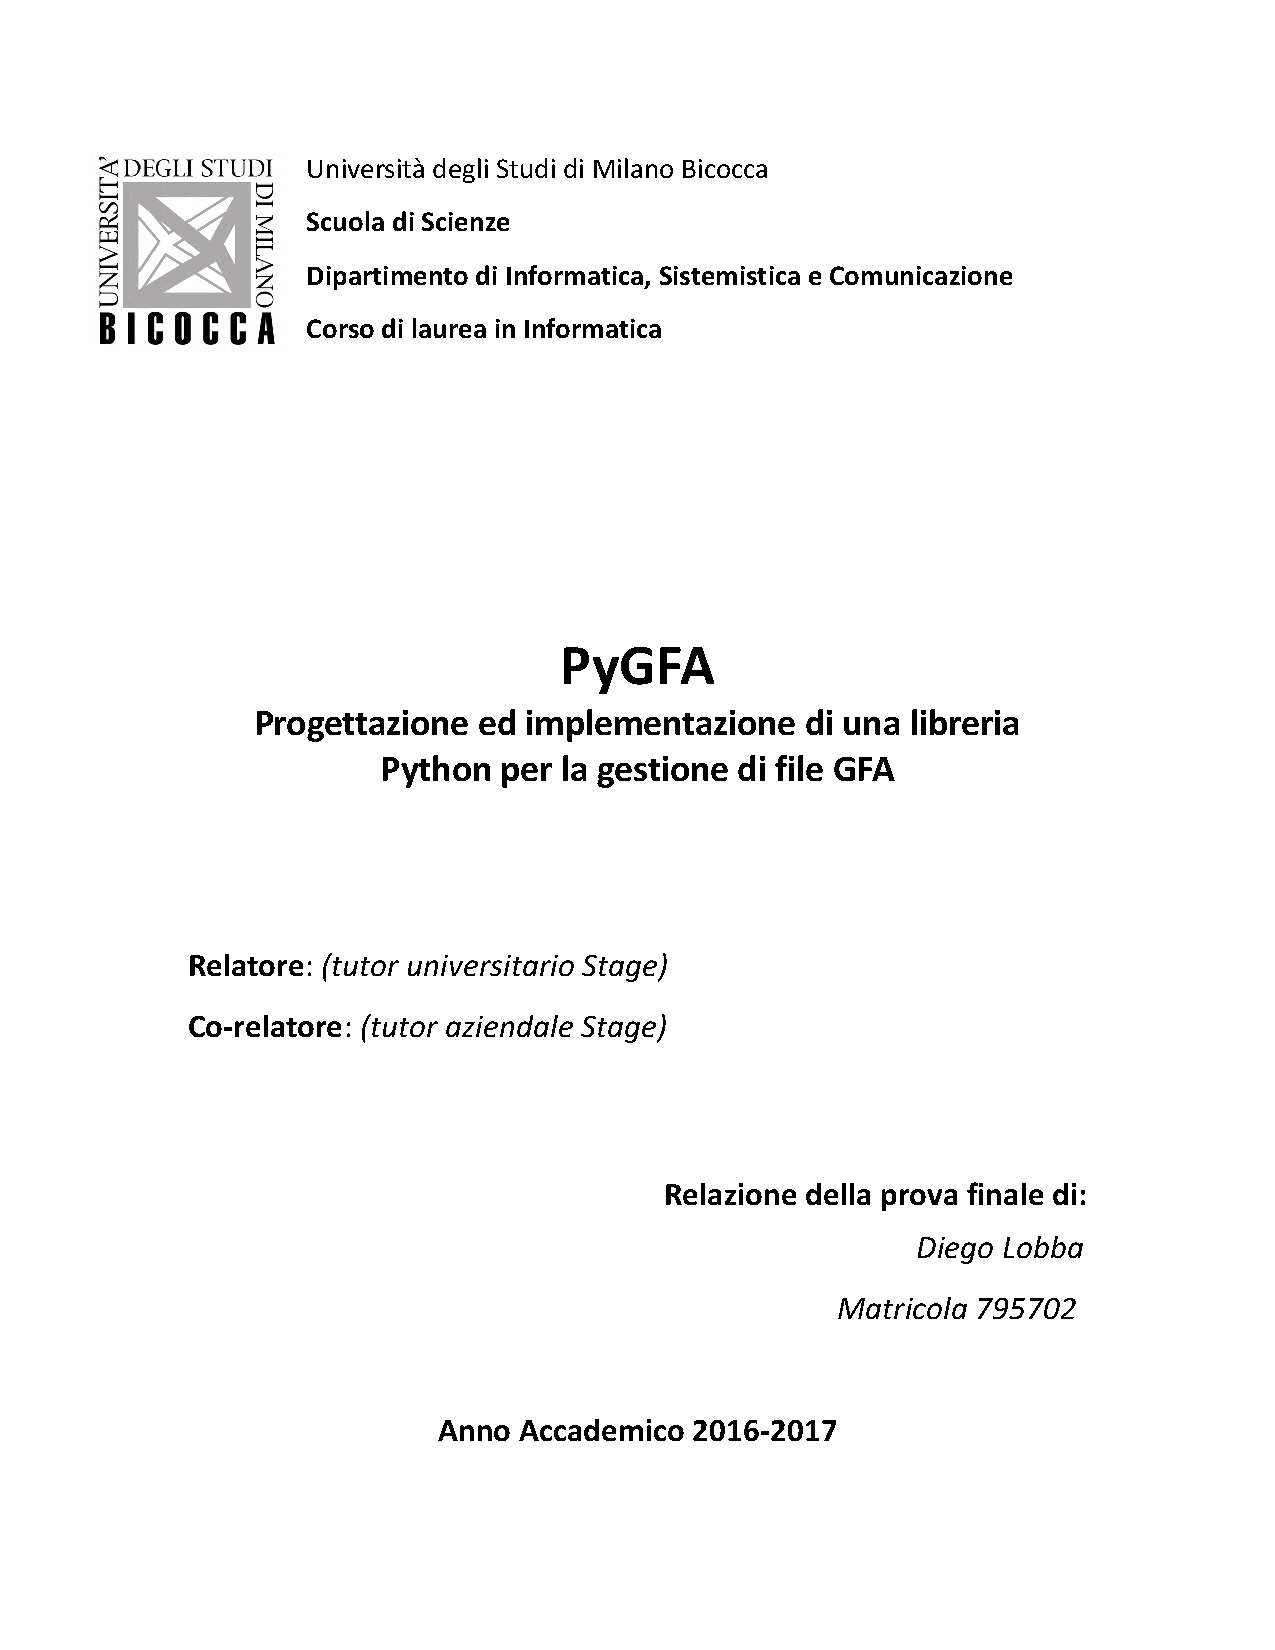
\includepdf[pages={1}]{immagini/frontespiziorelazionefinale20162017.pdf}

\tableofcontents
\listoffigures

\chapter{Introduzione}
\nocite{marx_2013}
Il DNA racchiude le informazioni che contraddistinguono gli organismi
viventi. Esso si può descrivere per mezzo di una stringa composta da quattro
lettere: A, C, G, T che denotano le quattro basi azotate (adenina, citosina,
guanina e timina rispettivamente) che costituiscono gli elementi
fondamentali del DNA stesso. Esso è un identificatore dello stato
corrente di un organismo, per questo lo studio delle sue variazioni
è di particolare interesse sia per l'identificazione di malattie,
che si possono manifestare come variazione di un particolare gene,
sia nel contesto evolutivo di una specie. A seconda delle necessità
è possibile sequenziare l'intero genoma di un organismo oppure estrapolare
le sole sequenze che ne codificano una parte, per esempio una proteina
particolare.

In principio la tecnica di sequenziamento del DNA più frequente era la tecnica
Sanger, in grado di restituire sequenze piuttosto lunghe (superiori al migliaio di
coppie di basi, indicate con il termine \emph{bp}) che permettono una ricostruzione
meno complessa dell'intero genoma di un organismo. Questa metodologia permette
di avere un'alta affidabilità sui dati ottenuti, ma ha degli alti costi d'utilizzo;
per questo motivo il metodo Sanger viene oggi solitamente utilizzato per
il sequenziamento completo di un DNA in casi particolarmente rari,
solitamente per specie dalle quali non si ha ancora un genoma di riferimento
o per la convalida di DNA ottenuti da metodi meno affidabili.

Negli ultimi anni si stanno diffondendo le cosiddette NGS (Next Generation Sequencing),
tecniche che permettono di ottenere una grande mole di dati
a prezzi molto ridotti, se confrontati con il metodo Sanger. Di contro questi
metodi producono sequenze di lunghezza inferiore, solitamente
intorno alle centinaia di coppie di basi, per questo motivo l'utilizzo di queste
tecniche non permette il sequenziamento efficace di DNA molto lunghi o che
presentano numerose ripetizioni, poiché il loro assemblaggio
risulterebbe poco affidabile.

Le sequenze ottenute da entrambi i metodi non è garantito
che siano le une contigue alle altre, di conseguenza è richiesto
l'uso di algoritmi di allineamento per individuare le parti sovrapposte
che denotano il proseguimento della stringa di DNA. Le informazioni
di questi allineamenti vengono salvate su file, seguendo una formattazione
ben definita, per poi essere processate
da programmi per l'assemblaggio del genoma.


I file GFA\cite{gfa_spec} (Graphical Fragment Assembly) sono file che descrivono	
questo tipo di informazioni. Ogni sequenza
viene vista come un nodo sul quale possono esserci collegate altre
sequenze per mezzo di collegamenti. Tali collegamenti possono
coinvolgere la sequenza secondo due direzioni:
\begin{itemize}
	\item la prima, indicata dal simbolo \textbf{+}, considera la
	sequenza così come appare nella sua definizione all'interno del file,
	\item la seconda, indicata dal simbolo \textbf{-}, considera la
	sequenza dopo che su di essa viene effettuata un'operazione di
	\emph{reverse and complement}.
\end{itemize}

I file GFA possono arrivare a contenere milioni tra sequenze e collegamenti
presenti tra di loro, per questo motivo si è voluto sviluppare una libreria, \pygfa,
in grado di gestire tali file permettendo non solo di andare ad effettuare
operazioni di filtraggio e selezione sulle informazioni contenute, ma
anche in grado di fornire una serie di strumenti per la loro
manipolazione ed ulteriore analisi.

\pygfa è una libreria Python che permette di gestire le informazioni
contenute in file GFA rappresentandole mediante una struttura a grafo.
La gestione delle operazioni sul grafo avviene sfruttando una libreria
preesistente: \emph{networkx}\cite{networkx}, per la quale vengono
fornite le interfacce ai metodi. \pygfa inoltre permette l'attraversamento del grafo mediante iteratori
personalizzati, che considerano solamente archi rappresentanti un
determinato tipo di connessione (\emph{dovetail overlap}) fra i nodi del
grafo.

\section{RGFA e GfaPy}
\pygfa non è la sola libreria che gestisce file GFA mediante una struttura a grafo.
RGFA è una libreria scritta in Ruby creata appositamente per questo scopo e GfaPy
è l'equivalente riscritta in Python. GfaPy non solo implementa le funzionalità di RGFA,
ma estende il supporto alla specifica GFA2 (che verrà successivamente illustrata).

Nonostante le somiglianze fra GfaPy e \pygfa, le due librerie non solo differiscono
a livello implementativo, ma hanno una gestione dei dati completamente diversa.
Le informazioni in GfaPy continuano a tenere informazioni sulla loro origine (il tipo
di linea dalla quale provengono). In \pygfa invece le informazioni vengono	
ricondotte ad un unico livello di astrazione; tutti i collegamenti possiedono
lo stesso numero di campi, i quali successivamente potranno averli definiti o meno
a seconda del tipo di linea/collegamento. Questo approccio di \pygfa è stato
preferito per tenere una coerenza generale nei dati usati dal grafo networkx
sottostante e per avere un'informazione che l'utente della libreria può interpretare
in senso più ampio; slegato dal concetto che la specifica GFA le assegna, ma
rappresentante il concetto biologico che tale informazione vuole significare.

\chapter{Ecosistema e strumenti}
\label{ch:ecosistema}
In questo capitolo verranno descritti i linguaggi utilizzati e gli
strumenti impiegati nell'analisi, nello sviluppo e nei test della libreria.
Di ogni elemento verrà fornita una breve panoramica, ponendo
maggior enfasi sugli aspetti (alle volte piuttosto tecnici) che è
stato necessario tenere in considerazione durante lo sviluppo
di \pygfa.

\section{Il linguaggio Python}
\nocite{wiki-python}
Python è un linguaggio di programmazione ideato da Guido van Rossum
all'inizio degli anni `90. Python è un linguaggio che si appresta a molteplici
stili di programmazione, sfruttando caratteristiche del paradigma object
oriented, funzionale e della programmazione strutturata.
Tali proprietà permetto l'uso del linguaggio in una grande varietà di attività:
nella creazione di script di automazione di sistema, nella scrittura di
sistemi web di backend fino allo sviluppo di complesse librerie di analisi numerica
e machine learning.

\begin{wrapfigure} {O} {0.35\textwidth}
	\begin{centering}	
		
\includegraphics{python-logo}
		\caption[Logo Python]{Logo del linguaggio di programmazione Python.}
	\end{centering}
\end{wrapfigure}
La minima struttura necessaria a produrre un programma Python,
l'inferenza del tipo delle variabili a runtime (\emph{dynamic typing}),
la gestione automatica della memoria e la sua espressività lo rendono
un candidato ideale nella prototipazione di sistemi nuovi, coerente con
processi di sviluppo agili e con la pratica di extreme programming.

Inoltre Python è un linguaggio interpretato, di conseguenza è possibile
effettuare, direttamente all'interno dell'interprete, verifiche in tempo
reale delle funzionalità attualmente in sviluppo.
Il fatto che il linguaggio venga interpretato
da un interprete permette una facile integrazione del codice nativo
con il quale l'interprete stesso è stato implementato.
Per questo motivo -e grazie al livello di astrazione sul quale si colloca-
esistono diverse implementazioni del linguaggio Python
che sfruttano la JVM, la piattaforma .NET, il linguaggio C o che si
concentrano maggiormente su alcuni aspetti specifici come la velocità,
il multithreading e la minimalità per l'uso in ambienti embedded.

\captionsetup{justification=centering, singlelinecheck=false}
\begin{lstlisting}[language=Python, frame=topline, caption=Un esempio  dell'espressività\\del linguaggio applicata a \pygfa.]
>>> import pygfa
>>> gfa = pygfa.gfa.GFA.from_file("data/sample1.gfa")
>>> gfa.nodes()
['1', '3', '2', '5', '13', '6', '11', '12', '4']
>>> pygfa.nodes_connected_components(gfa) #calcola i nodi
	di ciascuna componente connessa
...
[{'2', '1', '3', '6', '5'}, {'11', '13', '12'}, {'4'}]
>>> # estrai tutte le componenti connesse
	con numero di nodi maggiore di 3
...
>>> [component for component in pygfa.nodes_connected_components(gfa)
	if len(component) > 3]
[{'2', '1', '3', '6', '5'}]
\end{lstlisting}
\captionsetup{justification=justified, singlelinecheck=false}

\subsection{Classi, convenzioni e duck typing}
In Python per creare una classe è necessario definirla mediante
la dicitura:
\begin{lstlisting}[language=Python]
class MiaClasse(Antenata1, Antenata2, ...):
	...
\end{lstlisting}
Come è possibile notare, è ammissibile ereditare da più classi.
Tale caratteristica non è molto frequente negli altri linguaggi e
viene spesso considerata una cattiva pratica, visto che non
permette di accorgersi di una errata definizione della gerarchia delle
classi di progetto. Tuttavia, in Python questa proprietà permette
l'aggiunta di funzionalità alla classe, in modo analogo alla modalità
\texttt{implements} di Java, rendendo possibile una definizione di
quelle che in realtà sono le interfacce e le loro implementazioni.
In \pygfa tale funzionalità è stata applicata per aggiungere le
funzionalità degli iteratori personalizzati alla classe \texttt{GFA}.

Python è un linguaggio fortemente influenzato dai movimenti
open source; infatti ogni programma, libreria e sistema scritto in Python
presuppone che l'utilizzatore abbia libero accesso al sorgente e che
possa capire le modalità di utilizzo di ogni modulo di cui è composto.
Per questo motivo i programmi tendono ad essere ricchi di documentazione,
sia essa incorporata nel codice che allegata nel manuale.
Come conseguenza il linguaggio non offre un meccanismo per definire i
metodi di una classe come privati; in virtù del fatto che l'utilizzatore, avendo
la piena possibilità di capire il funzionamento del singlo modulo di sistema,
ha la piena responsabilità delle sue azioni.
Per aiutare a distinguere elementi del programma che l'autore vorrebbe
fossero non utilizzati (o utilizzati con particolare consapevolezza) si è
soliti nominare tali elementi facendo precedere i loro nomi da un singolo
trattino basso (\emph{weak internal use}). E' possibile imprimere
maggior enfasi nell'oscuramento di un elemento precedendo
il suo nome da due trattini bassi, in tal modo l'accesso
all'elemento avviene precendo il nome della classe al nome dell'elemento.

\captionsetup{justification=centering}
\begin{lstlisting}[language=Python, frame=topline, caption=Convenzioni per l'uso interno.]
>>> class A:
...	def __init__(self):
...		self.normal_use = 5
...		self._internal_use = 10
...		self.__strong_internal = 15
...
>>> a = A()
>>> a.normal_use
5
>>> a._internal_use
10
>>> a._A__strong_internal
15
\end{lstlisting}
\captionsetup{justification=justified}

Una ulteriore convenzione comune al Python e ampiamente considerata
nello sviluppo di \pygfa è il cosiddetto \emph{duck typing}.
Visto che il Python usa il binding dinamico, le funzioni e i metodi non
possono verificare il tipo dei parametri passati tramite signature.
Una possibile soluzione è verificare il tipo del parametro mediante
la funzione \texttt{isinstance}, come avviene per esempio quando
si cerca di effettuare il \emph{downcast} dalla classe antenata
ad una sottoclasse nei linguaggi in cui il binding avviene staticamente.
Per esempio tale pratica si verifica in Java quando si va ridefinire il metodo
\texttt{equal} di una classe, avente come signature un tipo Object rappresentante
l'istanza da confrontare ed effettuando il downcasting del parametro alla classe
attuale prima di effettuare i confronti fra le due istanze.

In Python invece viene considerata un'altra via. L'oggetto passato come
parametro viene confrontato direttamente con l'istanza e in caso
di errori (per esempio l'oggetto potrebbe non avere un parametro al quale
si sta accedendo), viene lanciata un'eccezione dalla quale si ritorna l'ineguaglianza
fra i due oggetti. Questo è ciò che si intende per duck typing.

Questo comportamento permette di avere delle classi molto flessibili,
visto che la compatibilità fra le classi viene garantita dall'uguaglianza
delle interfacce (se due oggetti sono diversi, ma in un determinato
contesto hanno lo stesso comportamento, allora possono essere considerati
simili); ma potenzialmente annulla la simmetria dell'operatore d'uguaglianza.
Di conseguenza, dati due oggetti $A$ e $B$ di classi diverse, si può
avere la situazione in cui $A = B$, ma $B \neq A$.

\subsection{Perchè è stato scelto Python}
Oltre alle caratteristiche spiegate precedentemente che rendono Python
un linguaggio flessibile, potente e anche divertente da usare, altri fattori
che motivano la sua scelta sono:
\begin{itemize}
	\item l'elevato numero di librerie disponibili, di strumenti che accompagnano
		e velocizzano lo sviluppo e la manutenzione di un progetto:
		analizzatori di sintassi, strumenti di test e ambienti per la
		generazione automatica della documentazione;
	\item la sua diffusione in ogni campo di applicazione, compreso
		quello bioinformatico, che è una delle principali motivazioni dello sviluppo
		di \pygfa;
	\item l'ampia documentazione sia della libreria standard che delle librerie esterne,
		con soluzioni a buona parte dei problemi di programmazione comuni,
		comportando un abbassamento dei costi e dei tempi di manutenzione e
		sviluppo dei sistemi.
\end{itemize}

% NetworkX
\section{NetworkX}
NetworkX è una libreria Python che permette di creare e gestire grafi.
Essa fornisce inoltre un'ampia collezione di algoritmi applicabili a grafi e
alberi: algoritmi di attraversamento, di cammini minimi, di analisi del
flusso; sui quali si basa per fornire informazioni topologiche
del grafo, come la presenza di cicli, di componenti connesse e di
punti di articolazione.

La libreria usa le liste di adiacenza per rappresentare i nodi e gli archi ad essi
collegati mediante tre dizionari Python nidificati.
Il primo dizionario contiene gli identificativi univoci di ogni nodo e come valore
ha un secondo dizionario con chiavi i nodi collegati ad esso mediante un
arco. Il valore di questi è a loro volta un dizionario che rappresenta
gli archi che collegano il nodo del primo dizionario con quello definito nel secondo.

\begin{wrapfigure} {O} {0.35\textwidth}
	\begin{centering}	
		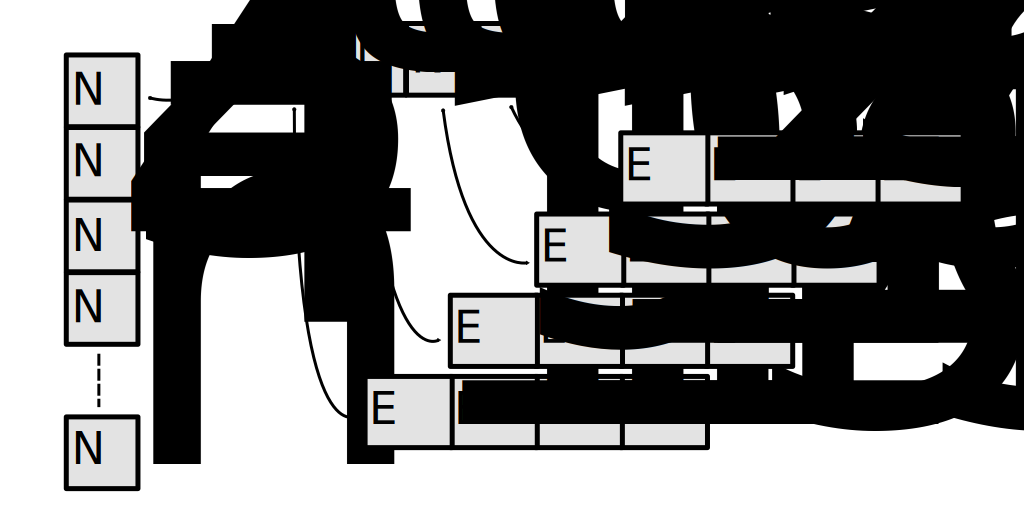
\includegraphics[scale=0.35]{networkx-dict}
		\caption[Rappresentazione nodi e archi networkx]{Rappresentazione grafica dei nodi e degli archi descritti in networkx.}
		\label{fig:networkx-dict}
	\end{centering}
\end{wrapfigure}

Questa scelta, oltre a rappresentare il modo più corretto per
implementare tale struttura\cite{python-graph}, permette un rapido
accesso ai nodi e agli archi che li mettono in relazione.

Oltre a specificare un identificativo univoco da assegnare a nodi e archi,
è possibile definire delle proprietà che possono essere dei tipi primitivi
o degli oggetti.

\subsection{Tipi di grafo}
Vi sono quattro differenti tipologie di grafo a disposizione:
\begin{itemize}
	\item grafo non diretto,
	\item grafo diretto,
	\item multigrafo non diretto,
	\item multigrafo diretto
\end{itemize}
Nel grafo non diretto, all'aggiunta di un arco $(u, v)$ tra
i nodi $u$ e $v$ viene aggiunto automaticamente un
arco $(v, u)$.

I multigrafi permettono di definire molteplici archi delimitati dalla
stessa coppia di nodi. In tal caso la definizione dell'identificativo
di un arco è di maggiore importanza, visto che sarà necessario
discriminare l'arco desiderato da un insieme di collegamenti
tra la stessa coppia di nodi. Per i multigrafi (diretti e non)
NetworkX permette, all'aggiunta di un arco, di specificare la chiave
(identificativo) associato all'arco che si sta inserendo; nel caso in cui
l'utente non definisce un identificativo, l'oggetto rappresentante il grafo
fornisce automaticamente un numero intero da assegnarli non ancora
utilizzato.

\subsection{Perchè è stata scelta e limiti}
\label{sec:nx-why-limits}
Il contenuto di un file GFA è direttamente rappresentabile mediante
un grafo, per questo sfruttare una libreria già esistente ha permesso
di velocizzare i tempi di sviluppo.

NetworkX offre la miglior implementazione dei grafi scritta in Python,
sfruttando dove richiesto librerie matematiche anche di basso livello
per garantire prestazioni molto alte in termini di velocità. La vasta
gamma di algoritmi a disposizione, uno sviluppo costantemente
attivo\cite{networkx-github} e un'ampia documentazione rendono
questa libreria un'ovvia candidata per lo sviluppo di \pygfa.

Uno svantaggio, dovuto all'implementazione direttamente in Python di
Networkx, è il consumo piuttosto elevato di memoria richiesto
per contenere il grafo. Tale peso è dovuto principalmente
all'uso dei dizionari come struttura di rappresentazione di nodi ed
archi. In \pygfa tale inconveniente è possibile notarlo specialmente
nei dizionari degli archi, che arrivano ad occupare più
di \SI{2}{\kilo\byte}.

Un altro aspetto negativo della libreria è che non permette l'impiego degli
algoritmi considerando le proprietà di archi e nodi. Ciò significa
che, supponendo di avere degli archi colorati (blu, giallo, rosso),
non è possibile applicare gli algoritmi solo agli archi di uno specifico
colore. Per questo in \pygfa si è reso necessario andare a ridefinire
(sfruttando il sorgente) gli algoritmi di interesse andando
a considerare nell'algoritmo i nodi definiti da un iteratore, che li
seleziona in base ad una proprietà dell'arco, evitando
di considerare l'intera lista di adiacenza del singolo nodo.

% Coverage.py
\section{unittest e Coverage.py}
Python è un linguaggio dinamico, per questo ogni
riga di un programma viene analizzata solo nel momento
in cui lo script viene lanciato. Ciò vuole significare che un errore
(esclusi quelli di sintassi) non può essere individuato prima
della sua esecuzione.

Per questo motivo nello sviluppo di \pygfa si è scelto di scrivere
i casi di test con la libreria \emph{unittest}, fornita direttamente
con l'interprete, e successivamente si sono andati ad analizzare
gli script dei casi di test con \emph{Coverage.py}.

Coverage.py è un programma Python in grado di misurare la
copertura del listato scritto, annotando le parti del codice che
sono state eseguite e creando un report (su file o su interfaccia web)
indicando le righe che necessitano ulteriore copertura.

Entrambi gli strumenti sono stati presi in considerazione per via
della loro facilità di integrazione nello sviluppo, per
la loro chiarezza nell'esposizione degli errori e delle statistiche
e per la loro diffusione tra gli sviluppatori.

\subsection{Funzionamento}
Lo strumento di analisi per la copertura prende in input un programma Python il quale
viene eseguito linea per linea. Tutti i file coinvolti nel programma
(poiché contenenti funzioni, classi o variabili usate presenti
nello script) vengono considerati nel calcolo della copertura. La
misura della copertura avviene sia per singolo file che sull'intero
insieme di file coinvolti dal programma. La copertura
sul singolo file viene calcolata come:
\begin{equation}
Cov(f) = \frac{\#linee_{coperte}}{\#linee_{totali}}
\end{equation}

unittest invece permette di confrontare il risultato di un'operazione rispetto
ad un valore atteso, fermando l'esecuzione nel caso in cui uno di questi
confronti fallisce. E' possibile inoltre confrontare il comportamento atteso
da una certa operazione, come l'invocazione di un'eccezione in caso di
operazioni non valide.

% Pylint
\section{Pylint}
\nocite{pylint}
Pylint è uno strumento di analisi del codice, curato dalla
Python Code Quality Authority\cite{pycqa}, in grado di applicare
una serie di regole atte a verificare:
\begin{itemize}
	\item la compatibilità del programma rispetto le convenzioni stabilite
		dal linguaggio\cite{python-pep8};
	\item problemi di importazione delle librerie;
	\item la presenza di variabili usate in un contesto in cui il loro valore
		sarebbe indefinito;
	\item il verificarsi di codice duplicato, sia all'interno dello stesso file
		sia fra sorgenti diverse.
\end{itemize}

Lo strumento quindi non solo fornisce dei meccanismi di standardizzazione
del codice, ma effettua quelle operazioni complementari a unittest e coverage.py
per la verifica della correttezza, da un punto di vista sintattico e simbolico,
del programma.

\subsection{Come è stato usato}

Pylint è uno strumento di \emph{controllo}, che fornisce suggerimenti riguardanti molti
aspetti del codice. Osservare tutti gli avvertimenti e risolvere tutti i problemi
rilevati avrebbe richiesto un prolungamento dei termini di consegna, oltre che
costituire un lavoro non prioritario.
Il suo impiego in \pygfa è voluto per cercare di uniformare una nuova libreria
Python con le convenzioni e le pratiche più comuni che la maggior parte degli
utilizzatori di questo linguaggio si aspettano, fornendo loro un ambiente
familiare nel quale la complessità non sia data dalla costante ricerca nella
documentazione di nomi e comportamenti insoliti circa elementi che compongono
la libreria. Generalmente si sono cercati di risolvere tutti quei problemi relativi gli standard
di nomenclatura oltre che problemi di analisi simbolica che avrebbero compromesso
il corretto funzionamento di \pygfa.

\addcontent{Indicare il numero di issue al momento della consegna di \pygfa.}

\section{Sphinx e Read the Docs}
\label{seq:sphinx-rtd}
Sphinx è uno strumento per la generazione automatizzata di documentazione
del codice. Grazie a questo strumento è possibile ricavare un manuale
ben formatto direttamente dal sorgente, il quale deve essere scritto
secondo un linguaggio ben specifico per indicare elementi di rilievo
del codice, come parametri, valori di ritorno, eccezioni,
note o link.

Sphinx è stato creato creato in origine per la documentazione ufficiale
del linguaggio Python\cite{python-doc} e fin da subito si è sparso
come strumento di aiuto nella documentazione di programmi scritti
non solo in questo linguaggio, ma anche in molti altri linguaggi supportati,
vista la sua flessibilità e i risultati ottimi che produce.

Esso usa il \emph{reStructuredText} come linguaggio di markup, permettendo
un'ampia espressività e una vasta gamma di notazioni come link (interni ed esterni),
definizione di tag personalizzati e liste (ordinate e non) oltre la possibilità
di scrivere formule matematiche in \LaTeX.

Sphinx permette di generare la documentazione finale nei formati più comuni:
HTML (con supporto mobile nativo), PDF e EPUB. Solitamente la scelta
più diffusa (che \pygfa segue) è quella di produrre la documentazione in
HTML e di renderla disponibile su \emph{Read the Docs}.

\phantomsection
\label{seq:sphinx}
Read the Docs è una piattaforma online, supportata dalla community,
appositamente pensata per salvare, catalogare e rendere disponibile
la documentazione scritta con Sphinx.
Il sito fornisce un ambiente Python e permette di collegare la documentazione
direttamente ad un repository di progetto su Github, evitando così di
dover mantenere aggiornate due copie di un singolo progetto separate.
Il sito usa l'ambiente Python per generare la documentazione di
progetto, permettendo di aggiungere le dipendenze del codice mediante
file di testo. La procedura è automatizzata (vedere figura
\ref{fig:rtd-build}) e il codice HTML risultante viene pubblicato sulla
piattaforma al termine del processo.

Grazie a Sphinx e Read the Docs è stato possibile documentare \pygfa
in modo facile e veloce, evitando di costruire soluzioni \emph{ad-hoc}
per la sua distribuzione e manutenzione e, allo tempo stesso,
si è riusciti ad ottenere un risultato più che accettabile utilizzando
i temi predisposti della piattaforma, garantendo all'utilizzatore
una facile consultazione sia da desktop che da mobile, una visione
del sorgente direttamente dalla documentazione e una funzione
di ricerca efficace.

\begin{figure}[h]
	\center
	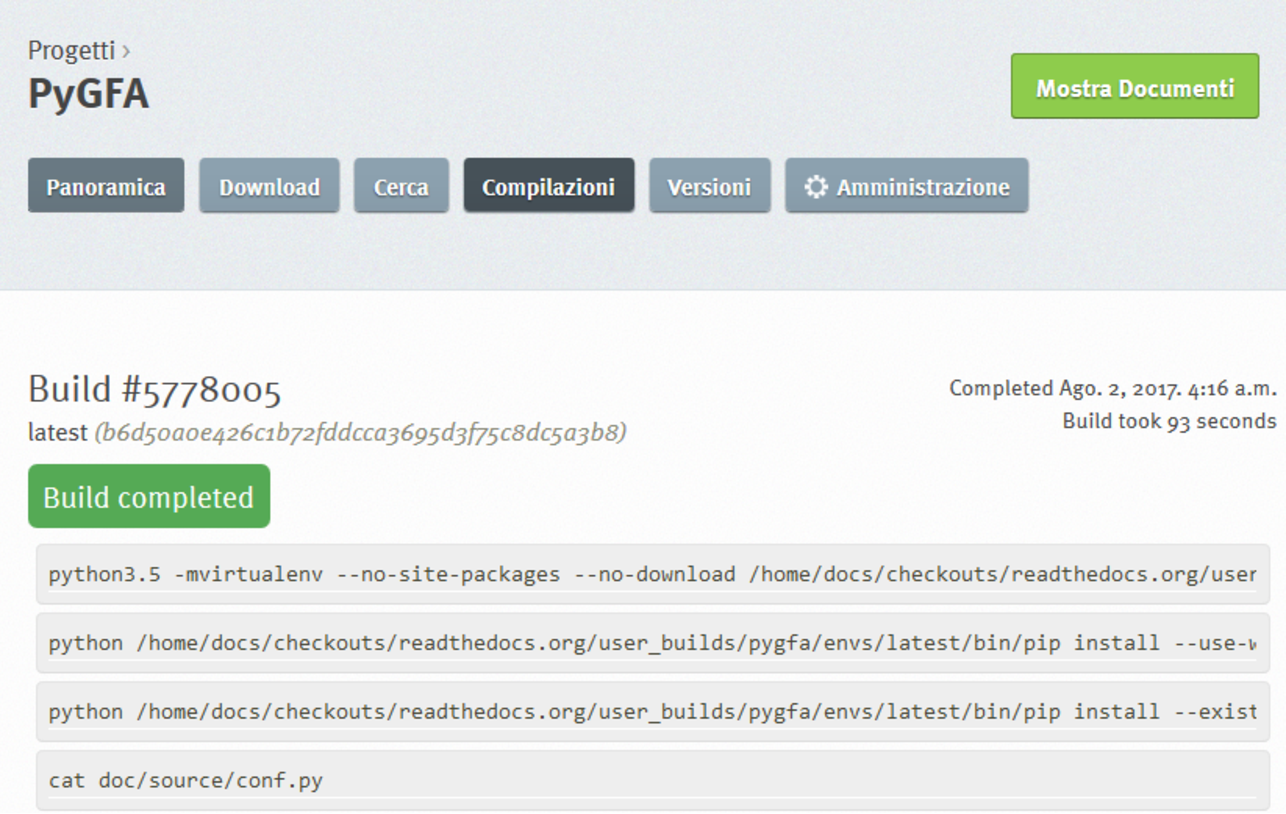
\includegraphics[scale=0.65]{rtd}
	\caption[Schermata di build di Read the Docs.]{Interfaccia per la generazione della documentazione in Read the Docs.}
	\label{fig:rtd-build}
\end{figure}

% git e GitHub
\section{git e GitHub}
\nocite{git}
\emph{git} è un sistema di controllo versione, ideato da Linus Torvalds per
gestire lo sviluppo del kernel Linux, tra i più utilizzati al mondo.
Esso permette di gestire progetti di ogni dimensione, garantendo velocità,
coerenza e ripristino fra le diverse tappe di sviluppo di un progetto.

\begin{wrapfigure} {O} {0.35\textwidth}
	\begin{centering}	
		
\includegraphics[scale=0.5]{git-logo}
		\caption[Logo git]{Logo dello strumento di controllo versione git.}
	\end{centering}
\end{wrapfigure}

Il programma permette, una volta inizializzato all'interno di una cartella,
di gestire i file in base ai cambiamenti ad essi effettuati. Per integrare
un cambiamento apportato ad un file è necessario aggiungerlo a quella
che viene chiama \emph{staging area}, contenente l'insieme
di file modificati a partire dall'ultimo stato aggiornato del sistema.
Generalmente i file nella staging area sono accomunati da un contesto
comune (una modifica che coinvolge per lo stesso motivo quello specifico
insieme di file), ma ai fini del sistema ciò non è un requisito indispensabile.
Terminate le modifiche e aggiunte alla staging area è necessario integrare
tali modifiche nel sistema mediante una \emph{commit}, un'operazione
che crea un identificativo univoco dello stato del sistema nel momento esatto
in cui i cambiamenti vengono integrati con esso. Grazie alla creazione
di questo identificativo è possibile ritornare nell'esatto stato
del sistema indicato, nel caso fosse necessario.

Git permette non solo di lavorare ad un progetto procedendo in un'unica
sequenza di sviluppo, ma permette la creazione di più diramazioni parallele
(\emph{branch}), indipendenti dalle future modifiche apportate al sistema,
che possono procedere nello sviluppo. Tali diramazioni garantiscono un
ambiente di lavoro isolato e stabile nel quale un singolo sviluppatore può
concentrare il suo sviluppo, senza preoccuparsi delle modifiche che altri
sviluppatori potrebbero apportare al sistema, per poi far ricongiungere
il componente nella principale sequenza di sviluppo (solitamente indicato
dal branch \emph{master}).

La flessibilità di sviluppo che questo strumento offre permette di strutturare
al meglio le diverse fasi di implementazione di un progetto, in piena coerenza con
un processo agile o di extreme programming. In \pygfa tale caratteristica
si è rivelata di fondamentale importanza, permettendo di suddividere
fasi di refactoring o di ridefinizione della struttura di progetto (operazioni
molto delicate da un punto di vista della stabilità della libreria) in un
ambiente controllato e reversibile in caso di problemi.

Completate le modifiche ed effettuata la commit, è possibile sincronizzare
i cambiamenti locali con una repository remota, un luogo decentralizzato
sul quale il lavoro viene salvato e grazie al quale è possibile condividere
il progetto con i propri collaboratori. Una tra le più famose piattaforme
che permettono di ospitare un repository git remoto è \emph{GitHub}.

GitHub è un sito che offre funzionalità paragonabili a quelle che Read
the Docs (vedi sezione \ref{seq:sphinx-rtd} a pagina \pageref{seq:sphinx})
fornisce per Sphinx. Permette di ospitare repository remote, catalogarle
per una maggiore accessibilità (se pubbliche) offrendo un'interfaccia
intuitiva per:
\begin{itemize}
	\item la creazione di \emph{tag} per il rilascio delle versioni stabili del sistema,
	\item la creazione di aree di discussione relative a bachi, miglioramenti e problematiche
		generali, fornendo agli sviluppatori un luogo centralizzato e coerente
		per la discussione di queste tematiche,
	\item lla creazione di punti di branching e analisi delle diverse ramificazioni del sistema
		e dell'attuale sequenza di sviluppo del progetto,
	\item la navigazione dell'intero progetto, con la possibilità di ispezionarlo
		ricreandone lo stato dopo una specifica commit,
	\item la visione di statistiche relative le commit effettuate da chiunque
		abbia contribuito al sistema, con la possibilità di analizzare le modifiche
		apportate a livello di singola commit.
\end{itemize}

Il ruolo che questi due strumenti hanno avuto e avranno nello lo sviluppo
di \pygfa è \emph{incalcolabile}. Non solo ai fini del salvataggio del
progetto, della sua gestione e della sua reperibilità, ma anche per la
possibilità che esso offre di permettere ad un qualsiasi sviluppatore di
effettuare facilmente una diramazione del codice ai fini di poterlo
riscrivere in base alle proprie necessità, senza doversi cimentare
nello sviluppo di un sistema nuovo (\emph{fork}).

% Bandage
\section{Bandage}
\label{sec:bandage}
\nocite{doi:10.1093/bioinformatics/btv383}
Bandage è un programma per la visualizzazione grafica di grafi
di assemblaggio. Questo strumento è in grado di visualizzare
grafi descritti da file GFA1, per questo il suo impiego
è stato di vitale importanza nell'analisi dei collegamenti presenti fra
le sequenze, specialmente nei casi di dovetail overlap, che descrivono
un continuum nel genoma e che per tanto costituiscono un'informazione
di rilievo per una libreria che si occupa della gestione di questi file.

\section{Conclusioni}
In questo capitolo sono stati presentati gli strumenti impiegati nello sviluppo
di \pygfa, nella fase di test e di documentazione indicando i dettagli
che si sono rivelati di particolare importanza ai fini implementativi del sistema.

% GFA specifications
\chapter{Le specifiche GFA}

In questo capitolo verrà fornita un'ampia panoramica sulle specifiche
GFA, sulle linee presenti e sulle diverse circostanze di assemblaggio
di sequenze che possono essere rappresentate.
Verrà inoltre fornita una breve introduzione ad alcuni concetti
biologici riguardanti gli elementi che compongono DNA e RNA e
la loro struttura, necessarie a comprendere le diverse situazioni
descritte nelle specifiche.

\section{Introduzione a GFA, motivazioni e struttura}
GFA è l'acronimo per Graph Assembly Format, è un
formato per la rappresentazione dei legami presenti fra le sequenze di
un genoma al fine di riuscire a ricostruirne la struttura.
Le motivazioni che risiedono alla base della proposta per un nuovo
formato consistono nell'uniformare le notazioni che programmi
di visualizzazione, di assemblaggio e di manipolazione potessero
utilizzare.

La prima versione della specifica GFA viene indicata col termine
GFA1. Questa prima versione, come vedremo successivamente,
limita la descrizione delle possibili situazioni in cui due sequenze
possono trovarsi in relazione. Per questo motivo, e per estendere
maggiormente l'insieme delle informazioni utili da descrivere,
è stata sviluppata una seconda specifica, indicata con GFA2.
Questa specifica generalizza, usando un'unica notazione,
i collegamenti fra sequenze descritti da GFA1 e permette inoltre
di descrivere relazioni di ogni tipo fra due sequenze.
GFA2 è un \emph{superset} di GFA1 e come tale permette
(con un minimo numero di operazioni) di trasformare un file GFA2
nell'analogo (rappresentabile) in GFA1. Questa seconda specifica
è stata appositamente pensata per permettere la descrizione di
sequenze e collegamenti imponendo un minimo numero di vincoli,
permettendo all'utilizzatore di impiegarla per la descrizione di dati
indipendentemente dai dettagli che questi forniscono.

Entrambe le specifiche adoperano la stessa formattazione delle linee.
Una linea descrive un'informazione di assemblaggio, sia
essa una sequenza, un collegamento o un insieme di elementi.
In ogni riga, il primo carattere indica
l'identità della linea stessa alla quale seguono, separati esclusivamente
da tabulazioni, gli elementi che costituiscono l'informazione
che la linea descrive e che prendono il nome di \emph{campi}.
I campi possono essere definiti o meno, nel qual caso l'assenza
dell'informazione viene indicata con un asterisco \texttt{*}.

In ogni linea di entrambe le specifiche è possibile descrivere campi
opzionali (che possono essere predefiniti per una linea o introdotti
direttamente dall'utente), descritti nel formato \texttt{TAG:TIPO:CONTENUTO}
dove \texttt{TAG} è una sequenza di due caratteri alfanumerici
(in maiuscolo se il campo è predefinito dalla linea, in minuscolo
altrimenti) che identifica l'informazione che esso indica.
Il \texttt{TIPO} di un campo viene anch'esso descritto da un
identificatore, ciascuno indicante il seguente contenuto:

\noindent
\begin{table}[h]
	\rowcolors{1}{white}{lightgray}
	\begin{tabularx}{\textwidth}{ | X | l | }
		\hline
		Tipo	&	Descrizione\\
		A 		&	Singolo carattere stampabile(escluso lo spazio)\\
		i 		&	Intero con segno\\
		f 		&	Decimale con precisione singola\\
		Z		&	Stringa stampabile (incluso lo spazio)\\
		J		&	Stringa JSON, escludendo caratteri di newline e di tabulazione\\
		H 		&	Array di Byte in formato esadecimale\\
		B 		&	Array di interi o di decimali\\
		\hline
	\end{tabularx}
	\caption{Tabella dei tipi che è possibile usare per specificare campi opzionali.}
	\label{tab:optfield-type}
\end{table}

\begin{wrapfigure} {O} {0.65\textwidth}
        \begin{centering}
                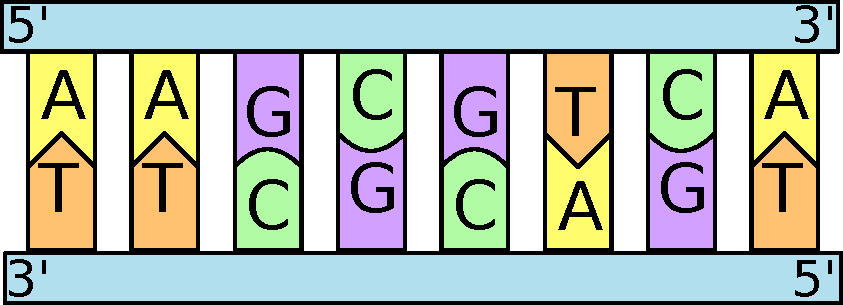
\includegraphics[scale=0.5]{dna-strand}
                \caption[Rappresentazione del DNA]{Rappresentazione grafica degli strand che compongono il DNA.}
                \label{fig:dna-strand}
        \end{centering}
\end{wrapfigure}

Mentre verranno analizzate le linee delle due specifiche, è essenziale
avere un'idea di cosa sia una sequenza e di come questa può essere in
relazione con le altre.
Con il termine sequenza viene indicata una \emph{sequenza nucleotidica},
un susseguirsi di lettere che denotano le unità molecolari che compongono
gli acidi nucleici di RNA e DNA (\emph{nucleotide}).
Una sequenza è priva di un ordine specifico, ma è possibile attribuirgliene
uno osservando la composizione del tipo di legame che collegano
gli elementi costitutivi il nucleotide, in base all'orientamento del
legame presente tra le unità di carbonio 3' di un un'unità
e la stessa unità 5' della successiva. Grazie a tale osservazione
è possibile individuare un ordinamento che verrà definito
come 5'3'.

Oltre questa considerazione, bisogna tenere conto che
l'informazione presente nel DNA
è la stessa a parità di estremità, ma in ordine inverso e
complementato (vedi figura \ref{fig:dna-strand}) (sostituendo
la citosina con la guanina e
l'adenina con la timina). Nel caso di RNA alla timina
si sostituisce l'uracile, ma il processo di formazione del RNA
prevede anch'esso questa operazione di complementazione
della sequenza.

Ergo, quando si considera una sequenza (nel caso
dell'assemblaggio del DNA), è necessario tenere presente
che un collegamento fra due sequenze potrebbe considerare
una sequenza posta sullo strand (una delle estremità
che compone l'elica del DNA) opposto e di conseguenza una loro
sovrapposizione potrebbe richiedere un preprocessamento della
stringa che la porti ad essere coerente con l'altra, operazione
che prende il nome di \emph{reverse and complement}.

% GFA1
\section{Linee GFA1}
GFA1 è la prima versione della specifica, essa si concentra nella descrizione
delle sequenze, collegate tra loro da una relazione di \emph{contenimento}
o di \emph{successione}.

Le linee previste dalla specifica sono header, segment, link, containment
e path.

L'header è una riga il cui scopo è quello di indicare la versione della specifica
in uso, può ripresentarsi più volte all'interno del file per indicare parametri
opzionali validi per tutti gli elementi. Tale linea viene indicata con il simbolo \texttt{H}.

\subsection{Segment}
La linea di Segment (indicata con il simbolo \texttt{S}) descrive in termini
generici una sequenza, la quale può essere definita o no. All'informazione
viene attribuito un identificativo che deve essere unico in tutto in file.
A queste proprietà se ne possono aggiungere altre, descritte da campi
opzionali, tra i quali la lunghezza (\texttt{LN}) e
il conto dei \emph{k-meri} (l'insieme di tutte le possibili sottostringhe
di lunghezza k contenute nella stringa).

\begin{lstlisting}[basicstyle=\ttfamily, caption=Una possibile Segment line.]
S	5	CCCGGGGTAA		LN:i:10
\end{lstlisting}

\subsection{Link}
\label{sec:link}
I Link (indicati dal simbolo \texttt{L}) sono il principale
tipo di relazione fra due sequenze. Essi
indicano una sovrapposizione fra le sequenze indicate da due Segment.
Nello specifico, un Link fra due Segment indica che la parte terminale
della prima sequenza è coinvolta in una sovrapposizione (\emph{overlap})
con l'inizio della seconda; il termine che descrive esattamente questa situazione
è \emph{dovetail overlap} tradotta in sovrapposizione a coda di rondine.
Tale tipologia di collegamento costituisce
un'informazione di rilievo nell'analisi dell'assemblaggio poiché descrive
un susseguirsi fra due sequenze.

Il link non solo descrive questa situazione, ma indica anche quale
estremità della sequenza è coinvolta nel overlap. Ricordando che
l'informazione contenuta nella struttura elicoidale del DNA è la stessa a parità
di estremi (ma in senso inverso e complementata), è possibile
che due sequenze siano contigue (in una situazione di dovetail
overlap) considerando la loro provenienza da due estremità
diverse dell'elica (strand).
Il link permette di esprimere il collegamento considerando anche questa
particolarità; per farlo esso utilizza un segno ``\texttt{+}'' per indicare
che la sequenza non necessita di alcun processamento nel suo
coinvolgimento nella sovrapposizione, mentre utilizza un segno ``\texttt{-}''
per esplicare la necessità di effettuare un' operazione di reverse
and complement sulla sequenza prima di poterla considerare
nel overlap.

Visto che, come si diceva poc'anzi, un Link descrive una sovrapposizione
tra la fine della prima sequenza e l'inizio della seconda (indipendentemente
dai segni associati alle due sequenze coinvolte), ciò da luogo a quattro
possibili situazioni:
\begin{itemize}
	\item la parte destra della prima sequenza si sovrappone con la parte
		sinistra della seconda (vedi figura \ref{fig:dov-ov}\subref{fig:dov-ov++});
	\item la parte destra della prima sequenza si sovrappone con la parte
		destra della seconda (vedi figura \ref{fig:dov-ov}\subref{fig:dov-ov+-});
	\item la parte sinistra della prima sequenza si sovrappone con la parte
		sinistra della seconda (vedi figura \ref{fig:dov-ov}\subref{fig:dov-ov-+});
	\item la parte sinistra della prima sequenza si sovrappone con la parte
		destra della seconda (vedi figura \ref{fig:dov-ov}\subref{fig:dov-ov--}).
\end{itemize}

\captionsetup{justification=centering}
\begin{figure}[h]
	\begin{subfigure}{.5\linewidth}
	  \centering
	  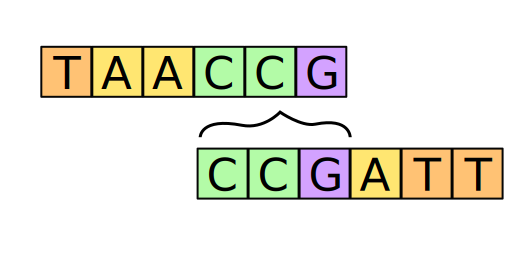
\includegraphics[scale=0.4]{dov_ov_++}
	  \caption{}
	  \label{fig:dov-ov++}
	\end{subfigure}%
	\begin{subfigure}{.5\linewidth}
	  \centering
	  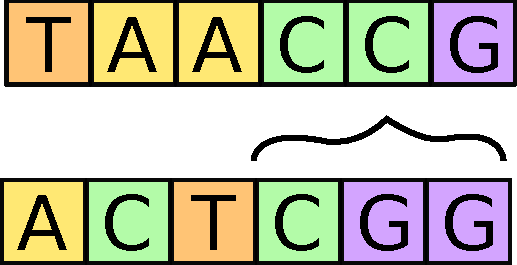
\includegraphics[scale=0.4]{dov_ov_+-}
	  \caption{}
	  \label{fig:dov-ov+-}
	\end{subfigure}%
	
	\bigskip%
	
	\begin{subfigure}{0.5\linewidth}
	  \centering
	  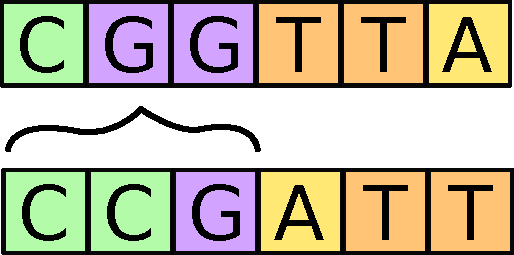
\includegraphics[scale=0.4]{dov_ov_-+}
	  \caption{}
	  \label{fig:dov-ov-+}
	\end{subfigure}%
	\begin{subfigure}{0.5\linewidth}
	  \centering
	  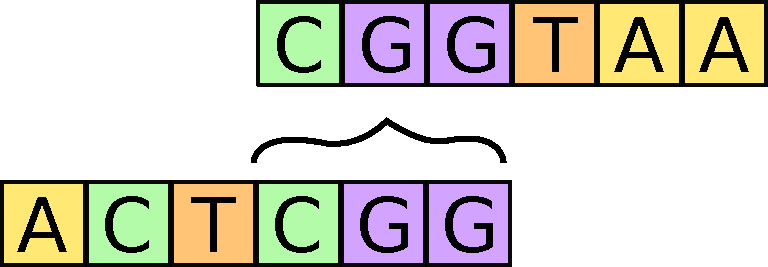
\includegraphics[scale=0.4]{dov_ov_--}
	  \caption{}
	  \label{fig:dov-ov--}
	\end{subfigure}
	
	\captionsetup{justification=justified}
	\caption[Rappresentazione delle possibili situazioni di dovetail overlap]{
		\textit{(a)} Dovetail overlap senza bisogno di alterare le sequenze.
		\textit{(b)}  Dovetail overlap dove la seconda sequenza necessita
	  		di un'operazione di reverse and complement per sovrapporsi alla prima.
	  	\textit{(c)} Un'operazione di reverse and complement deve essere eseguita
	  		sulla prima sequenza, affinché ci sia un overlap.
	  	\textit{(d)} Entrambe le sequenze richiedono operazioni di reverse and complement.}
	\label{fig:dov-ov}
\end{figure}
\captionsetup{justification=justified}

Oltre a questa considerazione sulle sequenze, il Link fornisce una descrizione
dell'allineamento, dato da una stringa CIGAR. Una stringa CIGAR è
una serie di lettere e numeri che descrivono lo stato di somiglianza
fra le due sequenze.
Tra i campi opzionali che il Link predispone si trova il campo
\texttt{ID}, mediante il quale è possibile riferirsi a tale
linea.
\clearpage

\subsection{Containment}
\label{sec:containment}
\begin{wrapfigure} {O} {0.35\textwidth}
	\begin{centering}	
		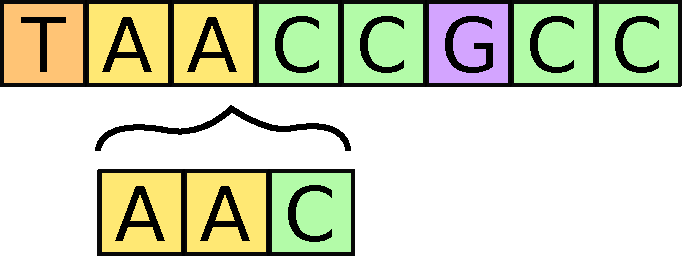
\includegraphics[scale=0.35]{containment}
		\caption[Rappresentazione di una situazione di contenimento fra sequenze]
		{Una rappresentazione grafica della situazione di contenimento fra due sequenze.}
		\label{fig:containment}
	\end{centering}
\end{wrapfigure}
Le linee di Containment (indicate con il simbolo \texttt{C})
descrivono sovrapposizioni fra sequenze nelle quali una stringa intera
è contenuta nell'altra.
I campi descrivono le stesse informazioni dei Link, ma è bene notare
i dettagli circa le posizioni delle sequenze che una sovrapposizione di
questo tipo comporta.
Date due sequenze $s1$ ed $s2$, un Containment tra la sequenza $s1$ e la
sequenza $s2$ indica che la sequenza $s1$ \emph{contiene} la sequenza
$s2$. In tale situazione vuole significare che la sovrapposizione comincia
dal primo carattere della sequenza di $s2$ e continua fino all'ultimo
(vedi figura \ref{fig:containment}).

Oltre ai classici campi che descrivono i nodi indicanti le sequenze coinvolte,
il loro orientamento nella sovrapposizione e l'allineamento; queste linee hanno un campo
che indica la posizione di inizio della sequenza contenuta nella sequenza
contenitrice.

\subsection{Path}
Un Path (indicato dal simbolo \texttt{P}) descrive un susseguirsi di
sequenze collegate esclusivamente da Link. Indica pertanto un percorso
di sequenze contigue all'interno del grafo. Queste linee
indicano esclusivamente gli identificativi e l'orientamento delle sequenze
coinvolte nel percorso cui seguono l'insieme delle stringhe CIGAR relative
l'allineamento delle sequenze prese a due a due.

\newpage
\captionsetup{justification=centering, singlelinecheck=false}
\begin{lstlisting}[basicstyle=\ttfamily, frame=topline, caption=Un esempio di file GFA 1.]
H	VN:Z:1.0
S	11	ACCTT
S	12	TCAAGG
S	13	CTTGATT
L	11	+	12	-	4M
L	12	-	13	+	5M
L	11	+	13	+	3M
P	14	11+,12-,13+	4M,5M
\end{lstlisting}
\captionsetup{justification=justified, singlelinecheck=false}


\section{GFA2}
GFA2 come accennato in precedenza è un'estensione di GFA1, pensata
per fornire più libertà all'utente circa le informazioni che è possibile descrivere.
Le linee appartenenti a questa specifica non comprendono campi opzionali
predefiniti, l'utente è libero di definire i campi aggiuntivi che più ritiene opportuni
per la sua applicazione.


\subsection{Segment}
Queste linee sono analoghe ai Segment in GFA1, ai campi viene aggiunto
un numero intero per descrivere la lunghezza della sequenza.
La lunghezza non vuole essere l'esatta lunghezza della sequenza, ma
vuole indicare la grandezza che tale sequenza assume quando rappresentata
da un programma di disegno (come Bandage, descritto a pagina \pageref{sec:bandage}).
Nell'indicare le sequenze non viene più richiesto l'uso di caratteri IUPAC\cite{wiki:acid-notation},
la sequenza può essere descritta con un qualsiasi carattere stampabile,
nello specifico dal simbolo ``\texttt{!}'' al simbolo ``\texttt{\textasciitilde}''
della tabella ASCII.

\subsection{Edge}
\begin{wrapfigure} {O} {0.35\textwidth}
	\begin{centering}	
		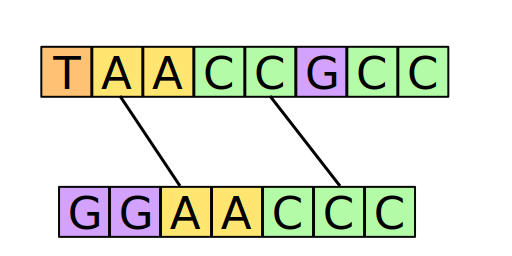
\includegraphics[scale=0.35]{generic-overlap}
		\caption[Rappresentazione di una situazione generica di sovrapposizione fra sequenze]
		{Una rappresentazione grafica di una generica sovrapposizione fra sequenze.}
		\label{fig:generic-overlap}
	\end{centering}
\end{wrapfigure}
La linea di Edge (indicata con la lettera \texttt{E}), indica un qualsiasi
tipo di sovrapposizione. Essa quindi generalizza le linee di Link e Containment
ed aggiunge la situazione in cui una generica parte di una sequenza
è sovrapposta ad una qualsiasi parte (non solo agli estremi) di
un'altra (come rappresentato in figura \ref{fig:generic-overlap}).

Questa linea, come Link e Containment, fornisce gli identificatori
delle sequenze coinvolte nel overlap e i rispettivi orientamenti, cui
si aggiungono le \emph{posizioni} di inizio e fine delle parti
delle rispettive sequenze sulle quali si svolge la sovrapposizione.
La posizione è un intero che parte da 0 (descrivendo il primo
carattere della sequenza) e termina in posizione pari alla
lunghezza stessa della sequenza, all'ultima posizione della sequenza
si pone il simbolo ``\texttt{\$}'', non farlo costituirebbe un errore.

In questo modo si avrà che una situazione di dovetail overlap
verrà indicata da un edge in cui le posizioni delle due sequenze
sono  $inizio1=0$ e $fine2=y\$$ o $fine1=x\$$ e $inizio2=0$;
mentre una situazione di contenimento viene descritta
da un edge in cui le posizioni delle sequenze sono $inizio1=0$ e 
$fine1=x\$$ o $inizio2=0$ e $fine2=y\$$. Si osservi che mentre
un contenimento in GFA2 non impone alcun ordine circa la sequenza
contenuta e quella contenitrice, un Containment in GFA1 prevede
che la prima sequenza sia la contenitrice e la seconda sia la contenuta;
inoltre in GFA2 non vi è alcun campo obbligatorio che indica l'inizio della
sequenza contenuta, diversamente da GFA1.

Come in GFA1 è possibile specificare l'allineamento, non solo mediante
stringa CIGAR, ma indicando una traccia DAZZLER (un indicatore
per eseguire l'allineamento fra sequenze in un tempo quasi lineare).
Quindi non solo GFA2 permette di descrivere la natura dell'allineamento tramite
CIGAR string, ma anche di descrivere un modo veloce per calcolarlo usando
le tracce DAZZLER. Come nelle altre situazioni delle specifiche, in caso
di mancata informazione viene posto un asterisco in tale campo.

Questa generalizzazione delle possibili sovrapposizioni tra due sequenze
permette di usare la specifica non solo per la descrizione di grafi di assemblaggio,
come nel caso di GFA1; ma anche di rappresentare, in un unico formato,
i risultati provenienti da diversi stadi del processo di assemblaggio.

\subsection{Fragment}
Le linee di Fragment (indicate con la lettera \texttt{F}) indicano un
collegamento fra una sequenza indicata nel file e una sequenza presente in un file esterno.
Il collegamento esprime un allineamento fra le due sequenze, in modo analogo ad
un Edge.

\subsection{Gap}
Le linee di Gap (indicate con la lettera \texttt{G}) indicano uno spazio
presente fra due sequenze, indicando la distanza che le separa e la
varianza di tale supposizione.

\subsection{Group}
I gruppi in GFA possono essere di due tipi, gli OGroup (indicati con la lettera \texttt{O})
e gli UGroup (indicati con la lettera \texttt{U}). I primi indicano una sequenza ordinata di elementi
GFA2 (escludendo gli UGroup) che individuano un percorso all'interno del grafo, mentre
gli UGroup indicano un insieme di elementi del grafo privi di ordine. Entrambi
i gruppi descrivono un sottografo che è possibile ricavare
dal grafo descritto dal file GFA.

\captionsetup{justification=centering, singlelinecheck=false}
\begin{lstlisting}[basicstyle=\ttfamily\scriptsize, frame=topline, caption=Un esempio di file GFA 2.]
S	1	122	*
S	3	29	TGCTAGCTGACTGTCGATGCTGTGTG
E	1_to_2	1+	2+	110	122$	0	12	12M
S	5	130	*
S	13	150	*
O	14	11+ 12+
S	11	140	*	xx:i:11
F	1	read1+	0	42	12	55	*	id:Z:read1_in_1
U	16	1 3 1_to_3
U	16sub	5 16
S	12	150	*
E	1_to_3	1+	3+	112	122$	0	12	10M
G	1_to_11	1+	11-	120	*
E	11_to_13	11+	13+	20	140$	0	120	120M
\end{lstlisting}
\captionsetup{justification=justified, singlelinecheck=false}

\section{Conclusioni}
In questo capitolo sono state esaminate le due versioni che costituiscono
la specifica GFA, indicando lo scopo del quale ciascuna versione intende
occuparsi e descrivendo i concetti che ciascuna linea vuole rappresentare
nel contesto dell'assemblaggio del genoma. Nel prossimo
capitolo si procederà nella descrizione del lavoro svolto nello sviluppo
di \pygfa \  e di come si è dovuto procedere nella rappresentazione delle
informazioni descritte nelle specifiche.

\chapter{Sviluppo}
In questo capitolo verrà descritto il processo di sviluppo
seguito per l'implementazione di \pygfa, analizzandone le
fasi principali, descrivendo i problemi incontrati e come sono stati
affrontati. Verrà infine fornito un caso di esempio che mostra
le funzionalità della libreria.

\section{Processo}
Lo scopo di \pygfa è quello di fornire un ambiente per lo sviluppo
di applicativi in grado di analizzare e manipolare file GFA. Non
è pertanto un prodotto finito, con casi d'uso definiti e risultati attesi
con cui è possibile confrontare i risultati. Non si è ritenuto appropriato,
di conseguenza, seguire un processo di sviluppo con fasi di analisi
e pianificazione profonde, che con il mutare dei requisti (per la
maggior parte non definiti fin dall'inizio) avrebbero potuto
compromettere la struttura del sistema. Un altro fattore da
tenere in considerazione è che le mie conoscenze sul significato
che i dati contenuti nei file GFA e le considerazioni che si potevano dedurre
da esse sono cresciute con lo sviluppo del sistema stesso. Perciò un'analisi,
anche se non approfondita, non poteva essere svolta a priori; poiché
avrebbe potenzialmente comportato una serie di ritardi
nello sviluppo del progetto dovute allo studio dei concetti biologici
che avrebbe richiesto diverso tempo.


Per questi motivi, il processo di sviluppo che si è deciso di utilizzare è di \emph{extreme}
\emph{programming}; con fasi di analisi e pianificazione molto veloci,
dando priorità all'implementazione delle parti essenziali del sistema aventi
maggior priorità per poi ripetere il procedimento con l'evolversi dei
requisiti e delle funzionalità richieste, cercando di avere un riscontro
costante con i clienti finali (in questo caso i referenti della tesi).

Affiancata alla parte di implementazione si è svolta la parte di testing,
che purtroppo non si è riusciti a condurre esattamente nella forma di Test Driven
Development, ma alla quale è stata data comunque una priorità molto alta
sia per la verifica delle funzionalità dei metodi, che per la verifica della
presenza di errori nel codice, che nel contesto di un linguaggio non compilato,
quale è il Python, risulta una pratica molto importante per garantire il
corretto funzionamento del programma.

Nel complesso si è riusciti a seguire abbastanza rigorosamente questi cicli
di pianificazione veloce, implementazione e test; procedendo al termine
di ogni ciclo con una fase di refactoring del codice e di miglioramento
della documentazione presente in esso, avvalendosi di Pylint per individuare
quelle porzioni di codice che era possibile migliorare.

\subsection{Fasi di sviluppo}
La rappresentazione delle informazioni contenute nei file GFA subisce
diverse trasformazioni prima di giungere come dato di un nodo, arco o
sottografo presente in un oggetto grafo GFA. L' iniziale rappresentazione
testuale di ogni linea viene rappresentata da una classe che ne indica
il tipo e i valori dei campi che contiene. Successivamente le linee
vengono convertite in archi, nodi o sottografi e infine nodi e archi
vengono rappresentati mediante dizionari Python, una volta inseriti
effettivamente nel grafo. Quest'ultima trasformazione è stata
adottata per uniformarsi al trattamento dei dati di un grafo in modo analogo
al modo in cui NetworkX li gestisce, garantendo una facilità di accesso
alle informazioni ed evitando che l'utente finale debba adattarsi ad un
nuovo modo di operare.

\'E possibile suddividere lo sviluppo di \pygfa in tre fasi principali:
\begin{itemize}
	\item sviluppo del parser;
	\item progettazione delle classi di astrazione dei dati GFA;
	\item sviluppo della classe del grafo GFA e delle operazioni che è
		possibile eseguire su di esso.
\end{itemize}
\captionsetup{justification=centering}
\begin{figure}[h]
	\centering
	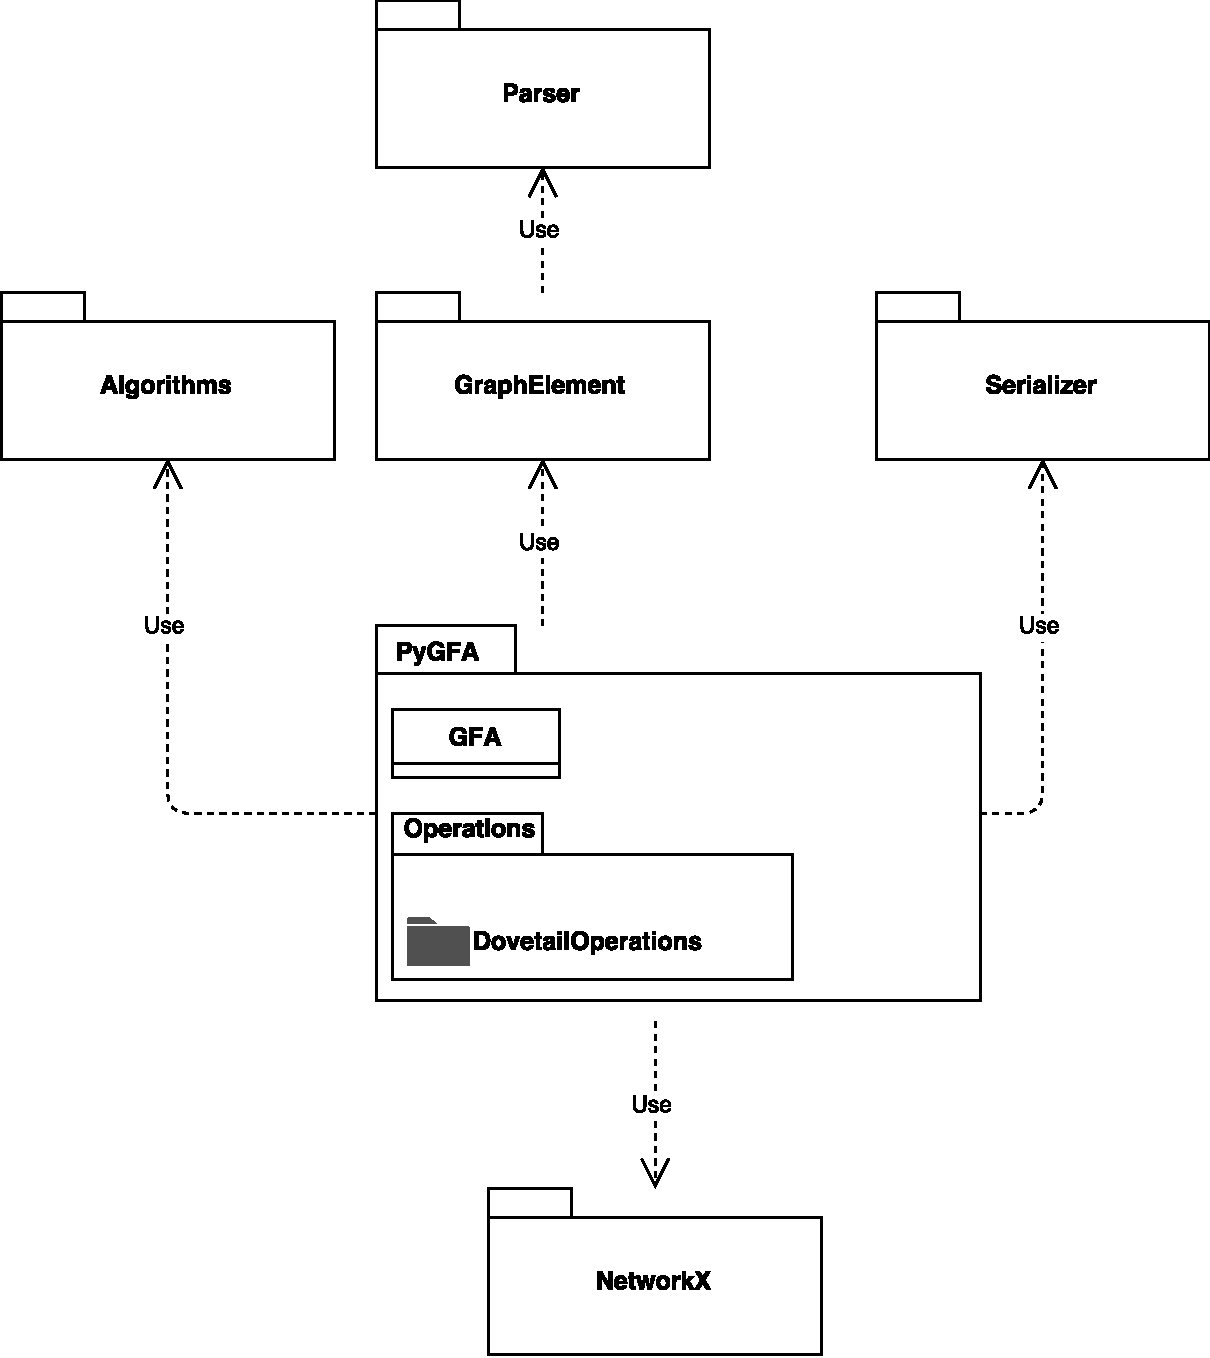
\includegraphics[scale=0.5]{package_diagram}
	\caption[Diagramma dei package]{Diagramma dei package di \pygfa.}
\end{figure}
\captionsetup{justification=justified}

Il parser si occupa di leggere le linee di un file GFA, di verificare la correttezza
sintattica dei suoi campi e di rappresentarne le informazioni mediante una classe
specifica per ogni tipo di linea.

Nella seconda fase si sono analizzate le linee delle due specifiche e si
è stabilito come attribuire ad ogni linea un ruolo che potesse essere di
nodo, arco o sottografo del grafo GFA finale. Gli attributi delle classi
del grafo astraggono gli attributi delle linee delle specifiche, 
di conseguenza è stata necessaria
una pianificazione dell'assegnamento degli attributi delle linee ad
attributi degli elementi del grafo.

Nella fase finale si è sviluppata la classe del grafo GFA fornendo
metodi di inserimento, accesso ed eliminazione sui singoli elementi che
lo compongono e aggiungendo le interfacce agli algoritmi forniti da Networkx
per eseguire le operazioni sui dati GFA.

\section{Fase1: sviluppo del parser}
Per la scrittura del parser si è seguito un approccio \emph{bottom-up},
sviluppando dapprima le classi rappresentanti i campi,
che sono presenti in ogni linea, 
e successivamente descrivendo con una classe ciascun tipo
di linea presente nelle specifiche.

Il parser effettua solo un controllo sintattico sulle informazioni dei file
al fine di garantire una corretta gestione delle informazioni da parte
della libreria; non verifica eventuali incongruenze tra le informazioni
presenti. Per questo motivo si suppone che il file GFA che viene fornito
sia stato già validato da un punto di vista di namespace degli elementi
e di coerenza delle informazioni (per esempio il riutilizzo di un identificativo
già utilizzato da un altro elemento o riferimenti a elementi
che non vengono definiti).

Ogni campo di ogni linea, in entrambe le specifiche, può essere descritto
da un \emph{espressione regolare}. Per questo motivo è stato
implementato un modulo Python per la validazione di tutti i campi definiti
dalle specifiche, associando un nome ad ogni espressione e creando un metodo
\texttt{is\_valid} che, data una stringa e il nome del tipo di un campo,
verifica che la stringa rispetti l'espressione regolare indicata dal nome
del campo fornito.
Per rappresentare i campi delle linee sono state create due classi,
\texttt{Field} e \texttt{OptField}; la prima
descrive i campi obbligatori, per i quali non viene specificato
esplicitamente il tipo di dato che contengono; la seconda
descrive i campi opzionali per i quali sono forniti
nome (il tag), tipo e valore. Mentre nei campi opzionali
è possibile, fin dall'instanziazione dell'oggetto, effettuare una validazione
sul contenuto, sui campi obbligatori non è possibile, in quanto
la tipologia del loro contenuto assume valore solo nel contesto
della linea cui appartengono.

Successivamente si è modellata la classe \texttt{Line} dalla quale
derivano le classi rappresentanti le altre linee. Questa classe
racchiude due campi: \texttt{PREDEFINED\_OPTFIELDS}
e \texttt{REQUIRED\_FIELDS} che racchiudono i campi opzionali che
ogni linea può contenere e i campi obbligatori che necessita, rispettivamente.
Inoltre questa classe possiede i metodi di aggiunta e rimozione dei campi,
assicurandosi di validare il contenuto dei campi obbligatori nel contesto
di ciascuna linea. Le altre classi, derivando da questa, devono
ridefinire i propri campi opzionali predefiniti e i campi obbligatori oltre
a indicare un metodo per convertire una stringa
nel corrispettivo oggetto che la rappresenta, condividendo la stessa
logica di manipolazione e validazione dei campi che viene riutilizzata
grazie al \emph{polimorfismo}.

\captionsetup{justification=centering}
\begin{figure}[h]
	\centering
	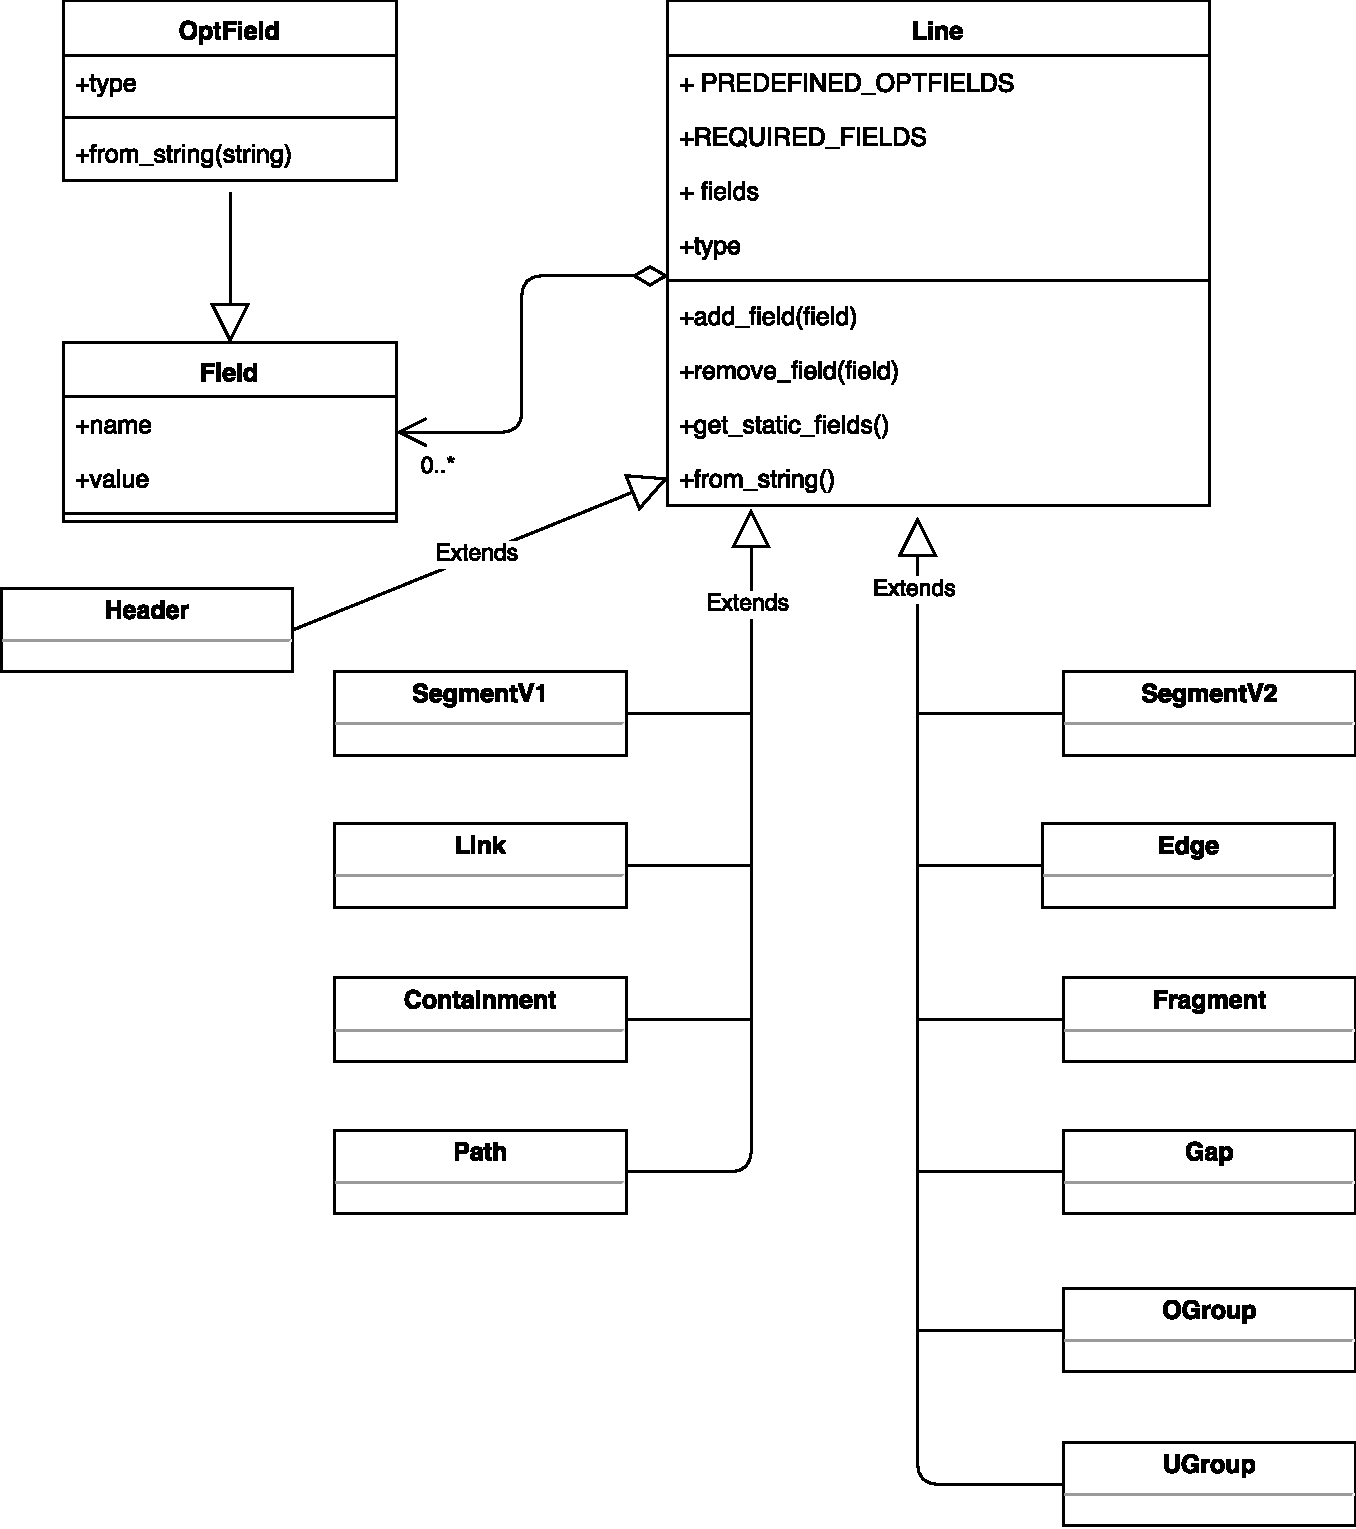
\includegraphics[scale=0.5]{parser_class_diagram}
	\caption[Diagramma delle classi del package parser]{Diagramma delle classi usate dal parser.}
\end{figure}
\captionsetup{justification=justified}
\clearpage

\section{Fase2: astrazione dei dati}
In questa fase sono state analizzate le singole informazioni presenti
nelle linee di entrambe le specifiche, evidenziandone gli aspetti simili al
fine di giungere ad una loro rappresentazione generalizzata per mezzo di tre
entità: \emph{Nodo}, \emph{Arco}, \emph{Sottografo}.

Ciascuna linea GFA può essere facilmente associata ad uno di questi tre
elementi. Nonostante sia possibile estendere GFA2 con nuovi tipi di linee, è bene notare
che questo lavoro di assegnazione di un ruolo ad ogni linea limita questa funzionalità
della specifica, in quanto sarebbe necessario capire il ruolo che queste nuove
linee possono ricoprire nei grafi di assemblaggio e ridefinire i meccanismi con
cui \pygfa riesce a manipolare queste nuove informazioni. \'E comunque possibile,
vista la mancanza dei concetti di visibilità privata del linguaggio, andare ad inserire
queste informazioni direttamente al grafo NetworkX che sta alla base dell'oggetto grafo
GFA, ma non è possibile garantire la consistenza delle operazioni che è possibile
effettuare usando la libreria.

Una sequenza costituisce il principale tipo di informazione cui si
è interessati, più sequenze sono in relazione da una serie di collegamenti descritti
dalle specifiche. Perciò possiamo attribuire alle sequenze (quindi alle linee Segment)
il ruolo di nodi.
La linea di header non contiene di per se informazioni che è possibile rappresentare
su di un grafo. Al momento \pygfa non modella le informazioni che possono essere
descritte dalle linee di header.

Tutte quelle linee che vedono come protagoniste due sequenze possono essere
considerate come degli archi che collegano due nodi $u$ e $v$. Appartengono
a tale insieme le linee di link, containment, edge, fragment e gap.

Le linee rimanenti: path, ogroup e ugroup, rappresentano tutte un insieme
(ordinato o meno) di nodi e archi che descrivono un sottografo composto
dagli elementi del file GFA; di conseguenza tali linee vengono considerate come
dei sottografi.

Visto che GFA2 è un superset di GFA1, si è analizzato come sarebbe stato
possibile rappresentare ciascuna linea di GFA1 nel corrispettivo elemento
di GFA2, capendo in questo modo gli attributi che ciascuna delle classi (Nodo, Arco
e Sottografo) avrebbe dovuto contenere per modellare quelle informazioni.
Terminato il confronto delle linee di GFA1 si sono aggiunte quelle
informazioni delle linee di GFA2 che non erano state prese in considerazione
(poiché non rappresentate) e le si sono andate ad aggiungere come attributi
aggiuntivi delle classi rappresentanti gli elementi del grafo.
Le informazioni che diventeranno attributi espliciti delle classi sono date
esclusivamente dai campi obbligatori di ciascuna linea, per entrambe le
classi i dati provenienti da campi opzionali verranno memorizzate
all'interno di un dizionario Python e indicate da un unico campo
\texttt{opt\_fields}; si noti che nonostante il nome, i campi contenuti
non sono (solamente) riferimenti ai campi opzionali delle specifiche,
ma si riferiscono ad una qualsiasi informazione
che l'utente vuole aggiungere all'elemento.

Di seguito verrà elencato ciascun campo di ogni linea, la relativa rappresentazione
in GFA2 e la scelta di come si è deciso di modellare tale campo nell'elemento
del grafo corrispondente. Per i nomi dei campi si farà riferimento alla nomenclatura
utilizzata dalla specifica per indicare ciascun campo, si noti
che alcuni nomi potrebbero subire variazioni in quanto la specifica è attivamente
in sviluppo e subisce continui cambiamenti. In questa tabella si fa riferimento
al nome dei campi così come si sono presentati al momento della fase dello
sviluppo.
Eventuali cambiamenti apportati negli ultimi periodi (entro la data indicata
dalla bibliografia) saranno indicati a piè pagina.

\subsection{Attributi della classe Nodo}
La classe nodo rispecchia senza aggiungere altre complicazioni
i campi descritti dalla linea GFA2 Segment.
Il campo \texttt{slen} che descrive la lunghezza della linea, nel
caso di GFA1, viene recuperato dal campo opzionale \texttt{LN};
nel caso non fosse specificato si cerca di ricavare tale valore
dalla sequenza stessa, calcolandone la lunghezza. Se la
sequenza non è specificata il dato assume valore \texttt{None}, per
indicare la mancanza di tale informazione.
\noindent
\begin{table}[h]
	\rowcolors{1}{white}{lightgray}
	\begin{tabularx}{\textwidth}{ | X | X | X |}
		\hline
		\textbf{Campo GFA1}	&	\textbf{Campo GFA2}	&	\textbf{Attributo nodo}\\
		Name				&	sid					&	nid (node id)\\
		Sequence				&	sequence				&	sequence\\
		Campo opzionale LN, lunghezza linea o \mbox{\textbf{None}}	&	slen	& slen\\
		\hline
	\end{tabularx}
	\caption{Tabella di analisi degli attributi del nodo.}
	\label{tab:node-analysis}
\end{table}


\subsection{Attributi della classe Arco}
Per determinare gli attributi della classe arco si sono dovuti analizzare i campi
di tutte le linee che potessero essere riconducibili ad un arco del grafo.

La prima linea da analizzare è stata la linea Link della specifica GFA1, la quale è
possibile ricondurla alla linea Edge di GFA2. Si nota dalla tabella \ref{tab:link-analysis}
l'esistenza di una corrispondenza uno a uno tra i campi della linea Link e quelli
della linea Edge. I campi della linea Edge contengono anche le posizioni
delle sequenze nelle quali si verifica l'overlap, ma tale informazione non è presente
nel Link di conseguenza questi quattro attributi dell'arco rappresentante un link
(beg1, end1, beg2 ed end2) saranno impostati a None.

\noindent
\begin{table}[h]
	\rowcolors{1}{white}{lightgray}
	\begin{tabularx}{\textwidth}{ | X | X | X |}
		\hline
		\textbf{Campo GFA1}	&	\textbf{Campo GFA2}			&	\textbf{Attributo arco}\\
		Campo opzionale ID o	\mbox{\textbf{None}}				&	eid					&	eid (edge id)\\
		From				&	sid1 (escludendo il segno)		&	from\_node\\
		From Orientation		&	segno di sid1					&	from\_orn\\
		To					&	sid2 (escludendo il segno)		&	to\_node\\
		To Orientation			&	segno di sid2					&	to\_orn\\
		Alignment				&	alignment						&	alignment\\
		\hline
	\end{tabularx}
	\caption{Tabella di analisi degli attributi della linea Link.}
	\label{tab:link-analysis}
\end{table}

Lo stesso comportamento è stato usato con la linea di Containment. In questo
caso però il campo relativo la posizione di inizio della sequenza contenuta non
è indicata nell'equivalente linea GFA2 Edge, e tale informazione
si è rivelata deducibile dalle posizioni di inizio e fine dell'overlap
indicata dal Edge stesso, di conseguenza a questa informazione è stata attribuita
una priorità minore e si è scelto di inserirlo come ulteriore campo opzionale dell'arco (chiamandolo
\texttt{pos}),
in modo da non perdere l'informazione nella fase di serializzazione
del grafo GFA in formato testuale.

Analizzando le altre linee rimanenti in GFA2 (Edge, Gap e Fragment), oltre agli attributi
necessari a rappresentare i campi di GFA1, si sono aggiunti gli attributi per
rappresentare l'inizio e la fine delle posizioni che coinvolgono l'overlap rispettivamente
per la sequenza di partenza e di arrivo, inoltre l'analisi sulle linee di Gap
ha richiesto l'aggiunta di attributi relativi la varianza e la distanza che questa linea
descrive. L'unica particolarità da evidenziare è la mancanza di un campo
analogo ad \texttt{eid} per la linea Fragment.

Si noti che le informazioni, con questo livello di astrazione, rendono difficile distinguere
le linee di Link, da quelle di Edge e di Fragment (le linee di Containment si distinguono
per la presenza del campo \texttt{pos} all'interno dei campi opzionali dell'arco mentre
quelle di Gap hanno sempre definiti gli attributi di varianza e distanza che le altre linee
hanno impostate a \textbf{None}). In questo caso la distinzione fra queste linee avviene avviene come
segue: gli Edge e i Link avranno il simbolo di asterisco come
identificativo nel caso l'informazione sia mancante,  mentre i Fragment
non hanno alcun campo che descrive un identificatore che li referenzia, perciò
il loro campo \texttt{eid} sarà None. Fatta questa distinzione, le linee di Edge se necessario
possono essere distinte da quelle di Link per la mancanza delle informazioni
circa le posizioni del overlap fra le sequenze che i Link descrivono.

In aggiunta agli attributi dei campi, si è deciso di aggiungere altre
tre informazioni per ogni.
Queste informazioni riguardano nello specifico i Link e gli Edge che
rappresentano un dovetail overlap (cioè quegli Edge che descrivono un Link).
Per questo tipo di archi viene impostato un attributo booleano \texttt{is\_dovetail}
che viene posto a vero e successivamente con i valori degli orientamenti
delle sequenze e delle posizioni dell'overlap (per gli Edge) vengono impostati
due campi \texttt{from\_segment\_end} e \texttt{to\_segment\_end} che indicano
l'estremità delle sequenze (``from'' e ``to'', rispettivamente) che vengono
prese in considerazione dall'overlap. Nel caso degli archi che non presentano
questa situazione, l'attributo \texttt{is\_dovetail} è impostato a falso e
gli attributi riguardanti le estremità sono posti a None.

Questa scelta ha permesso di andare ad effettuare tutta una serie di operazioni
sul grafo di notevole importanza ai fini dell'assemblaggio del genoma, visto che
le sovrapposizioni di dovetail rappresentano un continuum fra sequenze.
Se non si fosse adoperata questa soluzione il livello di astrazione introdotto da \pygfa
nella rappresentazione dei dati sarebbe stato troppo elevato e non avrebbe
permesso di usare efficacemente tutta una serie di operazioni che avrebbero
avuto senso solo per collegamenti di questo tipo.

\subsection{Attributi della classe Sottografo}
Le linee che sono rappresentabili dalla classe Sottografo sono i Path,
gli OGroup e gli UGroup.

Gli OGroup sono l'equivalente GFA2 dei Path, indicando ogni elemento
e il suo orientamento, a differenza degli UGroup i quali non indicano il
segno degli elementi che lo compongono.

Visto che i due gruppi in GFA2 indicano un eventuale overlap direttamente
negli elementi che lo compongono, il campo \texttt{overlaps} del Path
è stato inserito (in modo analogo al campo \texttt{pos} del containment)
nei campi opzionali della classe, in modo che sia possibile senza ulteriori operazioni
ricondurre il dato alla sua descrizione testuale in formato GFA1.

\noindent
\begin{figure}[t]
	\centering
	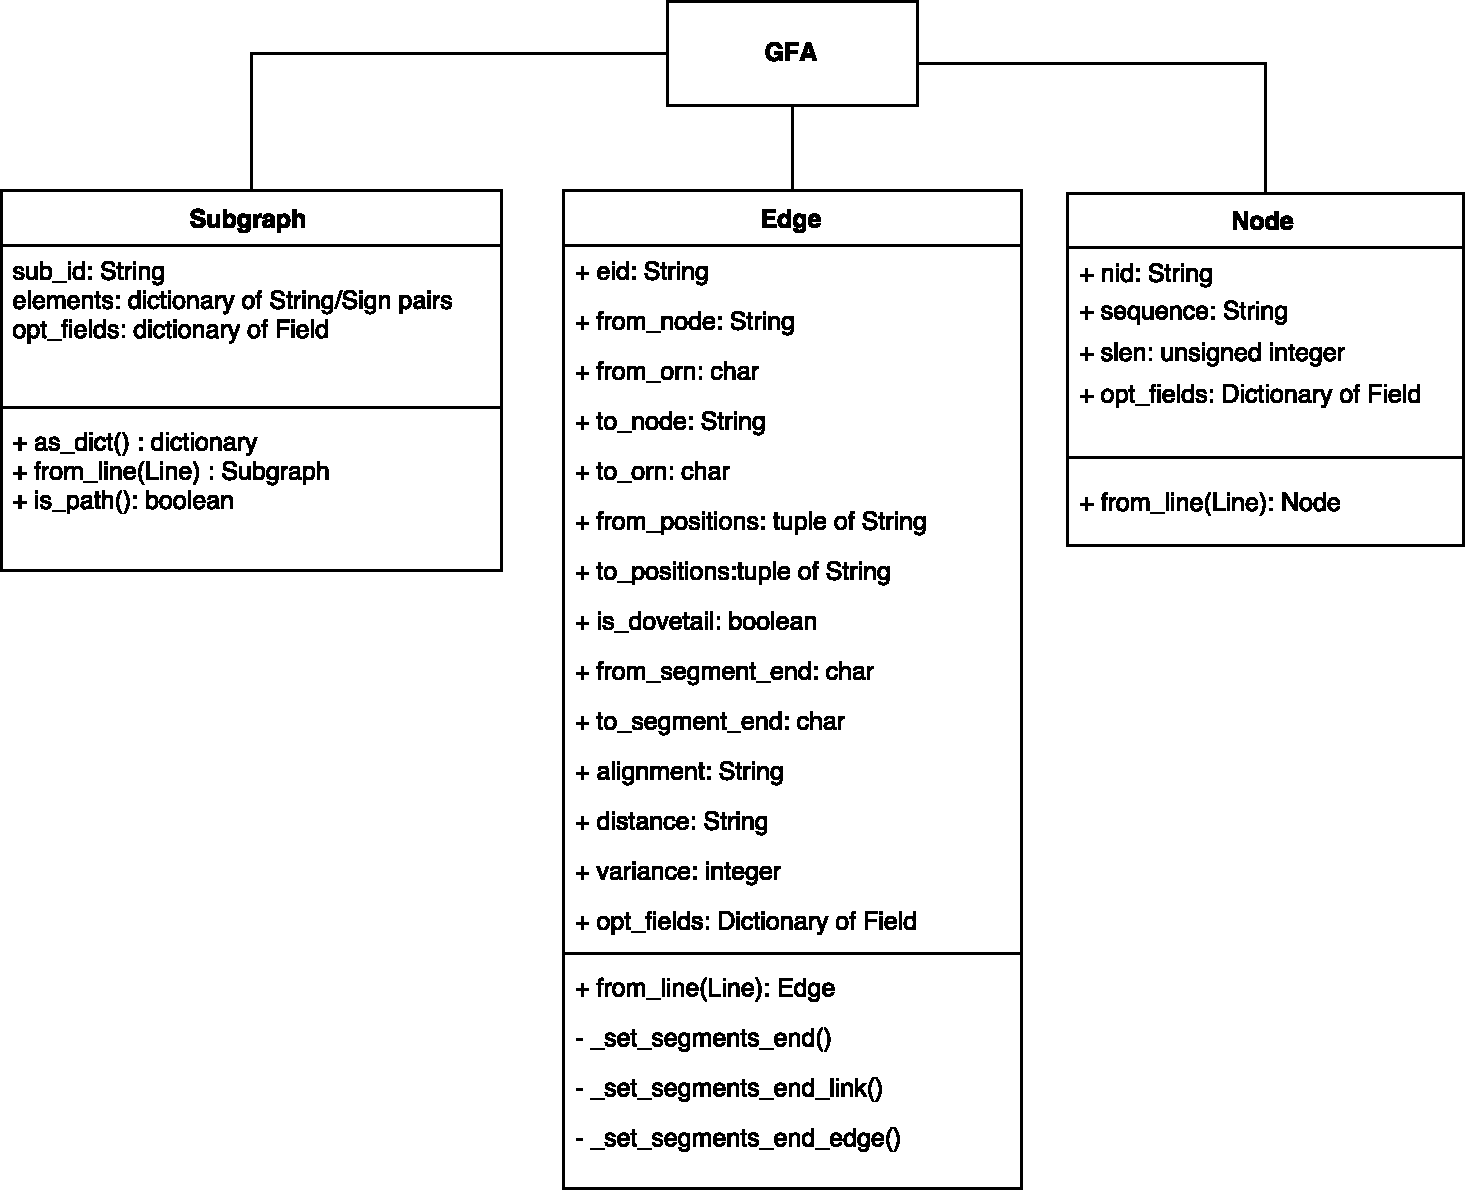
\includegraphics[scale=0.5]{graph_elements_class_diagram}
	\caption[Diagramma delle classi degli elementi del grafo]{Diagramma delle classi degli elementi del grafo.}
\end{figure}
\clearpage

\section{Fase3: rappresentazione del grafo GFA}
La classe che modella il grafo GFA sfrutta la classe Multigraph offerta
dalla libreria NetworkX come struttura ospitante gli archi e i nodi individuati
dalla fase precedente. Il multigrafo è stato scelto in quanto permette
di inserire più archi tra due nodi $u$ e $v$ inoltre
le relazioni presenti fra le sequenze non esprimono un senso di direzionalità
degli archi, perciò si è usato un grafo non diretto.
A nodi e archi è possibile inserire un qualsiasi tipo di riferimento ad un oggetto specificando
in fase di inserimento l'attributo del nodo al quale collegare il valore definito; la libreria
salverà l'informazione in un dizionario, di conseguenza il reperimento del valore
riferito al campo del nodo avverrà in modo analogo all'accesso ad un dizionario.

Per uniformarsi a tale comportamento \pygfa in fase creazione di nodi ed
archi estrapola gli attributi del elemento del grafo da inserire (in caso di nodo o arco)
e li inserisce sotto forma di coppia indice-valore di un dizionario. In questo modo
è possibile accedere facilmente ai diversi attributi di nodi e archi; inoltre
tale scelta è stata preferita in quanto questi elementi non hanno un comportamento,
ma rappresentano solamente un insieme di informazioni con relativi metodi di accesso.
di conseguenza sarebbe stato inappropriato descriverli mediante una classe.
\'E bene notare che ciò non vuole significare che le classi che modellano gli elementi
del grafo ricoprano un ruolo minore, esse sono servite ad astrarre informazioni
comuni ad elementi diversi tra loro riducendo quella complessità che altrimenti si
avrebbe avuto al momento di inserire nodi e archi nel grafo GFA.
I sottografi sono invece contenuti in un dizionario a parte, separato dalla struttura a
triplice dizionario rappresentata in figura \ref{fig:networkx-dict} a pagina \pageref{fig:networkx-dict};
il dizionario in questo caso contiene direttamente riferimenti ad oggetti Subgraph i quali
vengono convertiti in dizionari in base alle necessità dei metodi o dell'utente grazie
al metodo \texttt{as\_dict()}.

Per l'implementazione del grafo GFA si è scelto di usare la composizione al posto
di sfruttare l'ereditarietà della classe multigrafo. Tale scelta si è preferita per
un semplice concetto logico: la classe GFA \emph{sfrutta} un multigrafo senza
volerne emulare le funzionalità. Di conseguenza alla classe sono stati forniti i metodi di interfaccia
alla classe multigrafo oltre ad un metodo di accesso agli archi fornendo
solamente l'identificativo di un arco.

\subsection{Iteratore sugli archi di dovetail}
Come accennato a pagina \pageref{sec:link} le sovrapposizioni
che si sviluppano tra la fine di una sequenza e l'inizio di un'altra sono
informazioni di rilievo nel contesto dell'assemblaggio del genoma,
di conseguenza si è cercato di inserire una serie di meccanismi in \pygfa
che permettessero di distinguere gli archi che possiedono
il valore \texttt{is\_dovetail} a true, visto che NetworkX non fornisce
una soluzione a questa necessità (come descritto a pagina \pageref{sec:nx-why-limits}).

Questa funzionalità è stata implementata dalla classe \texttt{DovetailIterator} che
fornisce una serie di iteratori per scorrere i soli nodi del grafo collegati da archi di
dovetail overlap.
\noindent
\begin{figure}[t]
	\centering
	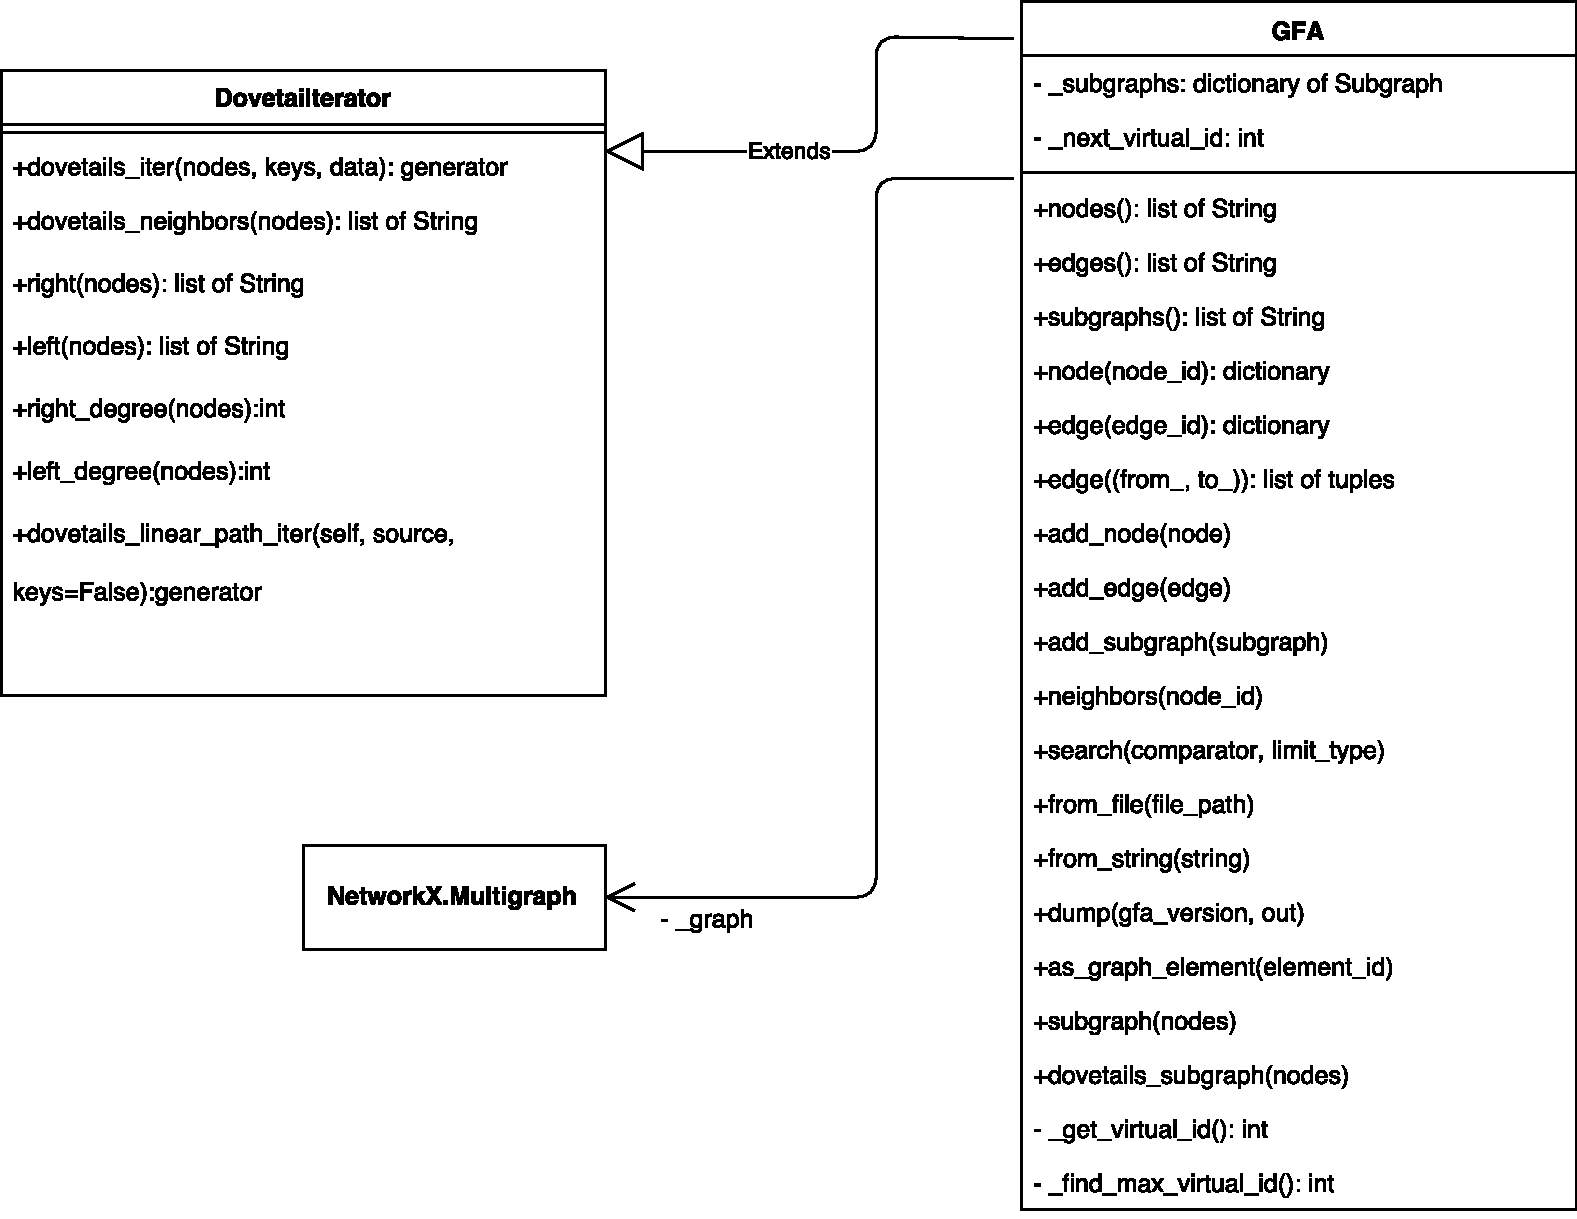
\includegraphics[scale=0.5]{gfa_class_diagram}
	\caption[Diagramma delle classi del grafo GFA]{Diagramma delle classi del grafo GFA.}
\end{figure}
\clearpage

\section{Operazioni sul grafo}
\pygfa offre una serie di operazioni che è possibile applicare sul grafo
composto da sequenze (nodi) e relazioni fra due sequenze (archi),
dividendole in due gruppi applicativi che si distinguono per le modalità
in cui gli archi vengono considerati nell'esecuzione delle operazioni.

Il primo insieme considera tutti gli archi del grafo, indistintamente dall'essere
archi di edge, fragment, gap o altro tipo. Queste operazioni sono
di utilità generale e servono per avere la massima flessibilità nella selezione delle
informazioni che il grafo contiene.

In questo gruppo troviamo il metodo della classe GFA \texttt{search} che
restituisce l'insieme di tutti gli elementi del grafo per i quali la funzione fornita
tra i parametri assume valore true. In questo modo l'utente definendo un
comparatore  può effettuare una serie di operazioni si ricerca e filtraggio sul grafo.

Inoltre, grazie all'uso della libreria NetworkX, è stato possibile con estrema facilità
creare delle interfacce ai metodi per l'individuazione delle componenti connesse, sia
per quanto riguarda la ricerca della componente connessa contente un nodo dato, che
la ricerca di tutte le componenti connesse presenti nel grafo.

Considerando l'alto livello di astrazione delle informazioni contenute
nel grafo, per l'utente che intende utilizzare \pygfa come strumento di
aiuto nella ricostruzione del genoma, è sconveniente andare ad eseguire
operazioni considerando archi che non sono di dovetail overlap, visto
che la relazione che essi descrivono è quella di maggior rilievo ai fini
dell'assemblaggio. Di conseguenza \pygfa come gfapy offre una serie
di operazioni che considerano esclusivamente archi di dovetail overlap.

\subsection{Operazioni sugli archi di dovetail overlap}
Gli algoritmi disponibili con NetworkX non permettono l'attraversamento
del grafo considerando le proprietà degli archi, non è quindi possibile
direttamente usare i metodi forniti come invece fatto per le operazioni
che considerano l'intero grafo (come già discusso a pagina \pageref{sec:nx-why-limits},
quando sono stati presentati i limiti della libreria). Nonostante questo inconveniente, vista
la natura open source di NetworkX e la licenza favorevole alla sua modifica
e distribuzione senza vincoli, è stato possibile modificare gli algoritmi necessari
per l'implementazione delle operazioni richieste. In tutti i casi l'unica modifica
richiesta per ottenere il risultato atteso consisteva nel modificare
l'elenco dei nodi considerati in fase di iterazione dell'algoritmo,
non più considerando l'intera lista di adiacenza del nodo selezionato
al ``livello'' corrente, ma prendendo in considerazione i nodi adiacenti
collegati da un arco di dovetail overlap. Visto che l'iteratore personalizzato
per l'attraversamento di questi archi è stato già sviluppato nella classe
DovetailIterator ed esteso dalla classe GFA, i metodi di iterazione
sono già forniti direttamente con il grafo GFA.

\noindent
\begin{lstlisting}[boxpos=t, numbers=left, language=Python, frame=t, caption=BFS in networkx., label=code:bfs-nx]
def _plain_bfs(G, source):
  G_adj = G.adj
  seen = set()
  nextlevel = {source}
    while nextlevel:
      thislevel = nextlevel
      nextlevel = set()
      for v in thislevel:
        if v not in seen:
          yield v
          seen.add(v)
          nextlevel.update(G_adj[v])
\end{lstlisting}

\captionsetup{justification=centering}
\begin{lstlisting}[boxpos=t, language=Python, numbers=left, frame=t, caption=BFS in \pygfa., label=code:bfs-pygfa]
def _plain_bfs_dovetails(gfa_, source):
  if source not in gfa_:
    return ()
  seen = set()
  nextlevel = {source}
  while nextlevel:
    thislevel = nextlevel
    nextlevel = set()
    for v in thislevel:
      if v not in seen:
        yield v
        seen.add(v)
        nextlevel.update(gfa_.right(v))
        nextlevel.update(gfa_.left(v))
\end{lstlisting}

I due listati rappresentano l'implementazione dell'algoritmo BFS (Breadth First Search) presente
nella libreria NetworkX (listato \ref{code:bfs-nx}) e l'equivalente implementato in \pygfa
(listato \ref{code:bfs-pygfa}). \'E possibile notare come l'unica differenza fra i due listati
è presente nella selezione dei nodi da considerare per la prossima iterazione, nelle ultime
righe di entrambi i listati; mentre in NetworkX viene considerata l'intera lista di adiacenza, in
\pygfa si sfruttano gli iteratori definiti in DovetailIterator per selezionare gli archi di dovetail overlap
presenti alle estremità del nodo.
Questo rappresenta una semplice modifica che si è dovuta effettuare per
implementare le operazioni di dovetail overlap, in alcuni casi le modifiche
hanno richiesto più tempo e l'analisi completa dell'operato dell'algoritmo (come nel
caso dell'algoritmo per la ricerca dei percorsi semplice fra due nodi),
ma nella maggior parte dei casi le modifiche richieste sono state semplici
ed intuitive.

Effettuando le modifiche sopra descritte è stato possibile sviluppare
le seguenti operazioni sugli archi di dovetail overlap:
\begin{itemize}
	\item ricerca delle componenti connesse;
	\item rimozione delle componenti connesse con lunghezza
		totale delle sequenze al di sotto di un determinato valore di soglia;
	\item rimozione delle estremità ``morte'', cioè tutti i nodi con
		grado di ingresso o uscita minore o uguale a 1 e la cui rimozione non causa
		la divisione di una componente connessa;
	\item ricerca degli insiemi di percorsi formati da unitig, cioè sequenze
		le cui estremità sono collegate ad una sola altra sequenza;
	\item ricerca di tutti i percorsi praticabili per arrivare da un nodo $u$ ad
		un nodo $v$.
\end{itemize}

\newpage
\section{Esempio}
Si andrà ora ad illustrare le funzionalità di \pygfa considerando il file GFA
contenente le informazioni nel listato \ref{code:gfa-es}, che visualizzato
con la libreria Matplotlib (strumento usato per la visualizzazione dell'intero grafo)
produce il risultato in figura \ref{fig:plot-matplot}; si sottolinea che tale libreria
considera il contesto biologico associato alle informazioni, ma visualizza
solamente gli elementi del grafo e la loro disposizione.
Per visualizzare il grafo con Bandage, in grado di visualizzare solo archi Link di GFA1,
il file GFA1 equivalente è stato ottenuto usando la funzione \texttt{dump}
di \pygfa, la quale è in grado di convertire le informazioni del grafo GFA
in una delle due specifiche.
Il risultato finale è in figura \ref{fig:plot-bandage}, si
può notare come i Gap (per esempio quello tra s8 ed s11)
non sono visualizzati da questo strumento.

\captionsetup{justification=centering, singlelinecheck=false}
\begin{minipage}{\linewidth}
\begin{lstlisting}[basicstyle=\ttfamily\scriptsize, frame=topline, label={code:gfa-es}, caption=Il file GFA2 usato per l'esempio.]
S	s1	10	*
S	s2	10	*
S	s3	10	*
S	s4	10	*
S	s5	10	*
S	s6	10	*
S	s7	10	*
S	s8	10	*
S	s9	10	*
S	s10	10	*
S	s11	10	*
S	s12	10	*
S	s13	10	*
S	s14	10	*
S	s15	10	*
S	s16	10	*
E	ls1s2	s1+	s2+	7	9$	0	2	*
E	ls2s4	s2+	s4+	7	9$	0	2	*
E	ls1s3	s1+	s3+	7	9$	0	2	*
E	ls3s5	s3+	s5+	7	9$	0	2	*
E	ls4s6	s4+	s6+	7	9$	0	2	*
E	ls5s6	s5+	s6+	7	9$	0	2	*
E	ls6s7	s6+	s7+	7	9$	0	2	*
E	ls7s8	s7+	s8+	7	9$	0	2	*
E	ls9s10	s9+	s10+	7	9$	0	2	*
E	ls11s12	s11+	s12+	7	9$	0	2	*
E	ls12s13	s12+	s13+	7	9$	0	2	*
E	ls14s15	s14+	s15+	7	9$	0	2	*
E	ls15s16	s15+	s16+	7	9$	0	2	*
E	ls16s14	s16+	s14+	7	9$	0	2	*
G	gs1s9	s1+	s9+	15	*
G	gs8s11	s8+	s11+	15	*
\end{lstlisting}
\end{minipage}
\captionsetup{justification=justified, singlelinecheck=false}

\captionsetup{justification=centering, singlelinecheck=false}
\begin{figure}
	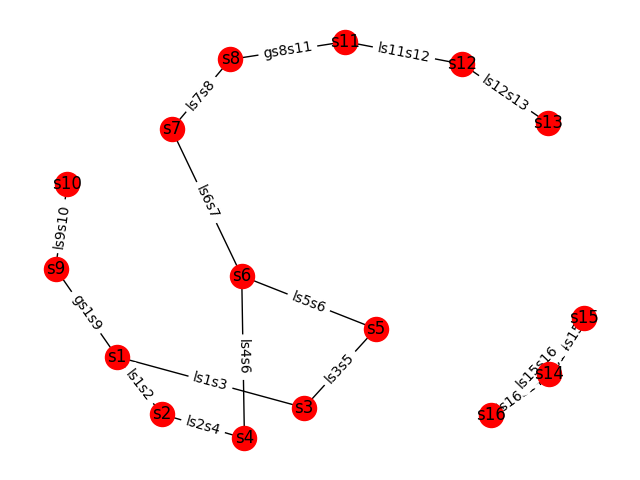
\includegraphics[scale=0.75]{matplot-es}
	\caption{Visualizzazione del grafo con matplotlib.}
	\label{fig:plot-matplot}
	\vspace{1cm}
	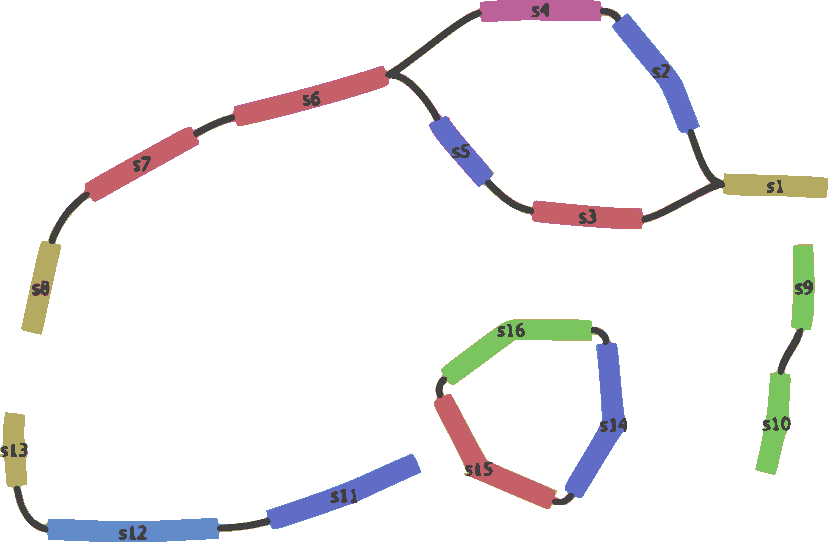
\includegraphics[scale=0.75]{bandage-es}
	\caption{Visualizzazione del grafo con Bandage.}
	\label{fig:plot-bandage}
\end{figure}
\captionsetup{justification=justified, singlelinecheck=false}

Caricato il grafo estraendo le informazioni dal file \texttt{gfa-es}
si andrà a presentare il modo in cui queste vengono rappresentate
mediante dizionari, si procederà successivamente
con la ricerca delle componenti connesse.
Si andrà ad illustrare l'operato degli iteratori personalizzati
cercando i segmenti collegati alle estremità di un nodo
specifico mediante l'uso i metodi \texttt{left} e \texttt{right}.
Si procederà quindi con le operazioni sugli archi di dovetail
individuando le componenti connesse e comparandole
con il risultato precedentemente ottenuto, per
poi concludere con i metodi per la ricerca
delle sequenze di unitig e dei cammini semplici
che si diramano tra due nodi $u$ e $v$.

\captionsetup{justification=centering, singlelinecheck=false}
\begin{minipage}{\linewidth}
\begin{lstlisting}[basicstyle=\ttfamily\scriptsize, frame=topline]
>>> import pygfa
>>> g = pygfa.gfa.GFA.from_file("..\..\gfa_es.gfa")
>>> g.nodes()
['s1', 's2', 's3', 's4', 's5', 's6', ..., 's15', 's16']
>>> g.node("s1")
{'nid': 's1', 'sequence': '*', 'slen': 10}
>>> g.edges(keys=True)
[('s1', 's2', 'ls1s2'), ('s1', 's3', 'ls1s3'), ..., ('s15', 's16', 'ls15s16')]
>>> g.edge(("s1", "s2"))
{'ls1s2': {'eid': 'ls1s2',
	'from_node': 's1', 'from_orn': '+', 'to_node': 's2', 'to_orn': '+',
	'from_positions': ('7', '9$'), 'to_positions': ('0', '2'),
	'alignment': '*', 'distance': None, 'variance': None,
	'is_dovetail': True, 'from_segment_end': 'R', 'to_segment_end': 'L'}}
>>> g.edge("ls1s2")
{'eid': 'ls1s2', 'from_node': 's1', 'from_orn': '+', 'to_node': 's2', 'to_orn': '+',
	'from_positions': ('7', '9$'), 'to_positions': ('0', '2'),
	'alignment': '*', 'distance': None, 'variance': None,
	'is_dovetail': True, 'from_segment_end': 'R', 'to_segment_end': 'L'}
>>> g.edge("ls1s2")["is_dovetail"]
True
\end{lstlisting}
\end{minipage}
\captionsetup{justification=justified, singlelinecheck=false}
La conversione degli elementi del grafo in dizionari ha permesso
una migliore integrazione nella libreria NetworkX facilitando l'accesso
alle informazioni del grafo. Di contro tale comportamento non permette di ricalcolare
automaticamente le informazioni della linea rappresentata in caso di modifica, cioè
non avendo una classe non è possibile attribuire un comportamento nella
gestione delle informazioni. Questo vuole significare che l'utente è libero di modificare
le informazioni, ma è suo compito assumersi la responsabilità che le modifiche
siano coerenti con il resto dei dati.


\captionsetup{justification=centering, singlelinecheck=false}
\begin{minipage}{\linewidth}
\begin{lstlisting}[basicstyle=\ttfamily\scriptsize, frame=topline, breaklines=true]
>>> pygfa.nodes_connected_components(g)
<generator object connected_components at ...>
>>>  le componenti connesse vengono restituite 
... # come generatore python
... # una componenente alla volta.
... # Per poterle visualizzare
... # tutte in una unica soluzione e'
... # necessario inserirle in una lista Python	
...
>>> list(pygfa.nodes_connected_components(g))
[
	{'s4', 's13', 's10', 's1', 's2',
		's3', 's9', 's5', 's8', 's12',
		's11', 's7', 's6'},
	{'s14', 's15', 's16'}
]
\end{lstlisting}
\end{minipage}
\captionsetup{justification=justified, singlelinecheck=false}
I due insiemi presenti all'interno della lista individuano le due componenti
connesse come mostra la figura \ref{fig:plot-matplot}. Tutti i tipi di archi che collegano
due nodi vengono presi in considerazione in tale operazione.


\captionsetup{justification=centering, singlelinecheck=false}
\begin{minipage}{\linewidth}
\begin{lstlisting}[basicstyle=\ttfamily\scriptsize, frame=topline]
>>> g.node("s1")
{'nid': 's1', 'sequence': '*', 'slen': 10}
>>> g.neighbors("s1")
['s2', 's3', 's9']
>>> g.right("s1")
['s2', 's3']
>>> g.left("s1")
[]
>>> g.dovetails_neighbors("s1")
['s2', 's3']
\end{lstlisting}
\end{minipage}
\captionsetup{justification=justified, singlelinecheck=false}
Dato il nodo $s1$ i nodi adiacenti considerando tutti i tipi di archi sono
dati dal metodo \texttt{neighbors}, mentre le operazioni successive
operano considerando solo archi di dovetail. Il metodo \texttt{left} restituisce
tutte le seguenze in cui è presente un dovetail overlap con la parte
sinistra della sequenza selezionata ($s1$ in questo caso), mentre il metodo
\texttt{right} restituisce le sequenze in cui la sovrapposizione avviene con
la parte destra della sequenza. I nodi adiacenti ad $s1$, considerando solo
questo tipo di collegamenti fra nodi, sono un sottoinsieme dei nodi individuati
dal metodo \texttt{neighbors}.


\captionsetup{justification=centering, singlelinecheck=false}
\begin{minipage}{\linewidth}
\begin{lstlisting}[basicstyle=\ttfamily\scriptsize, frame=topline]
>>> list(pygfa.dovetails_nodes_connected_components(g))
[
	{'s4', 's2', 's1', 's3', 's5', 's6', 's8', 's7'},
	{'s9', 's10'},
	{'s13', 's12', 's11'},
	{'s16', 's14', 's15'}
]
\end{lstlisting}
\end{minipage}
\captionsetup{justification=justified, singlelinecheck=false}
Le componenti connesse considerando gli archi di
dovetail sono più numerose rispetto quelle trovate
senza fare distinzione fra i legami dei nodi. Infatti si può
notare che gli archi di gap $(s9, s1)$ e $(s8, s13)$ non sono
presi in considerazione, facendo così aumentare il numero
totale delle componenti connesse. 


\captionsetup{justification=centering, singlelinecheck=false}
\begin{minipage}{\linewidth}
\begin{lstlisting}[basicstyle=\ttfamily\scriptsize, frame=topline]
>>> g.dovetails_linear_path_iter("s3")
<generator object DovetailIterator.dovetails_linear_path_traverse_edges_iter at ...>
>>> list(g.dovetails_linear_path_iter("s3"))
[('s3', 's5')]
>>> list(pygfa.dovetails_linear_paths(g))
[
	[('s4', 's2')],
	[('s15', 's14'), ('s14', 's16')],
	[('s13', 's12'), ('s12', 's11')],
	[('s9', 's10')],
	[('s5', 's3')],
	[('s7', 's8')]
]
>>> list(pygfa.dovetails_linear_paths(g, keys=True))
[
	[('s4', 's2', 'ls2s4')], 
	[('s15', 's14', 'ls14s15'), ('s14', 's16', 'ls16s14')],
	[('s13', 's12', 'ls12s13'), ('s12', 's11', 'ls11s12')],
	[('s9', 's10', 'ls9s10')],
	[('s5', 's3', 'ls3s5')],
	[('s7', 's8', 'ls7s8')]
]
\end{lstlisting}
\end{minipage}
\captionsetup{justification=justified, singlelinecheck=false}
L'iteratore sulle sequenze di unitig è un metodo
della classe GFA che restituisce gli archi che costituiscono il percorso
lineare contenente il nodo indicato come parametro.
La funzione per ricercare tutti i percorsi lineari sfrutta
gli iteratori sugli unitig per cercare l'insieme di tutte le sequenze
di unitig presenti nel grafo; alle tuple di nodi che compongono gli archi
che denotano i percorsi lineari è possibile associare anche il nome specifico
degli archi, in modo da distinguerli in presenza di più archi tra due nodi.


\captionsetup{justification=centering, singlelinecheck=false}
\begin{minipage}{\linewidth}
\begin{lstlisting}[basicstyle=\ttfamily\scriptsize, frame=topline]
>>> list(pygfa.dovetails_all_simple_paths(g, "s2", "s7"))
[
	['s2', 's1', 's3', 's5', 's6', 's7'],
	['s2', 's4', 's6', 's7']
]
>>> list(pygfa.dovetails_all_simple_paths(g, "s2", "s7", edges=True, keys=True))
[
	[('s2', 's1', 'ls1s2'), ('s1', 's3', 'ls1s3'),
		('s3', 's5', 'ls3s5'), ('s5', 's6', 'ls5s6'),
		('s6', 's7', 'ls6s7')],
	[('s2', 's4', 'ls2s4'), ('s4', 's6', 'ls4s6'),
		('s6', 's7', 'ls6s7')]
]
>>> list(pygfa.dovetails_all_simple_paths(g, "s2", "s11"))
[]
\end{lstlisting}
\end{minipage}
\captionsetup{justification=justified, singlelinecheck=false}
Nell'esempio si vogliono trovare tutti i percorsi che congiungono
il nodo $s2$ al nodo $s7$, la funzione ritorna le liste dei nodi che individuano
i percorsi di congiunzione. Impostando l'attributo \texttt{edges}
a True la funzione ritorna le sequenze di archi dei percorsi.
Nel caso non sia presente un percorso fra i due nodi specificati, la funzione
ritorna un generatore privo di elementi, che viene convertito
dalla funzione \texttt{list} in una lista vuota.


\chapter{Benchmark}
In questo breve capitolo verranno mostrati
alcuni risultati di \pygfa \  evidenziando il tempo di calcolo
richiesto per alcune delle operazioni che la libreria fornisce e misurando
lo spazio di memoria richiesto per l'immagazzinamento del grafo.
Verranno infine presentati dei grafici che evidenziano il
confronto con la libreria Gfapy in termini di tempo di esecuzione
e di spazio occupato.

Tutte le operazioni sono state effettuate su una macchina virtuale
Linux 64bit con le seguenti caratteristiche:
\begin{itemize}
	\item \SI{8}{\giga\byte} di ram;
	\item processore host da \SI{3.7}{\giga\hertz} quad-core, il
		sistema guest sfrutta due soli core;
	\item hard disk magnetico.
\end{itemize}

Le misure sono state effettuate su grafi generati casualmente
da uno script usato nello sviluppo di Gfapy; il programma
crea una serie di nodi collegati tra loro da sovrapposizioni
a coda di rondine, il risultato viene salvato in un file GFA1.
Visto che i grafi sono generati casualmente è improbabile
che si riesca a ripresentare la stessa configurazione di componenti
connesse e sequenze di unitig (a meno di salvare i file generati),
mentre il numero di nodi e archi rimane prestabilito al ripetersi
dei test. Per \emph{elementi del grafo}, nel contesto dei grafici presentati,
si intendono l'insieme di nodi e archi del grafo.
Per automatizzare la misurazione delle performance è stato
scritto un programma che si occupa di generare automaticamente
i grafi, effettuare le misurazioni, salvare i risultati su un file di testo
e rimuovere i grafi creati al termine.

Le operazioni che si sono andate a misurare sono:
\begin{itemize}
	\item il tempo impiegato per effettuare il parsing del file contenente il grafo;
	\item il tempo richiesto per ottenere i dizionari contenenti i nodi e gli archi;
	\item il tempo per calcolare le componenti connesse (sia considerando
		solo archi di dovetail sia considerando tutti i tipi di archi)
		\footnote{In questo caso, visto che lo script genera solo archi a coda
		di rondine, le componenti connesse individuate saranno le medesime. Si tenga
		comunque a mente che il tempo misurato riguarda il calcolo di entrambi
		i tipi di componenti connesse.};
	\item il tempo richiesto per la ricerca delle sequenze di unitig.
\end{itemize}
Oltre alla misura di questi tempi si è andato a misurare il consumo
di memoria necessario per contenere il grafo GFA.
\clearpage

\captionsetup{justification=centering, singlelinecheck=false}
\begin{figure}[h]
\centering
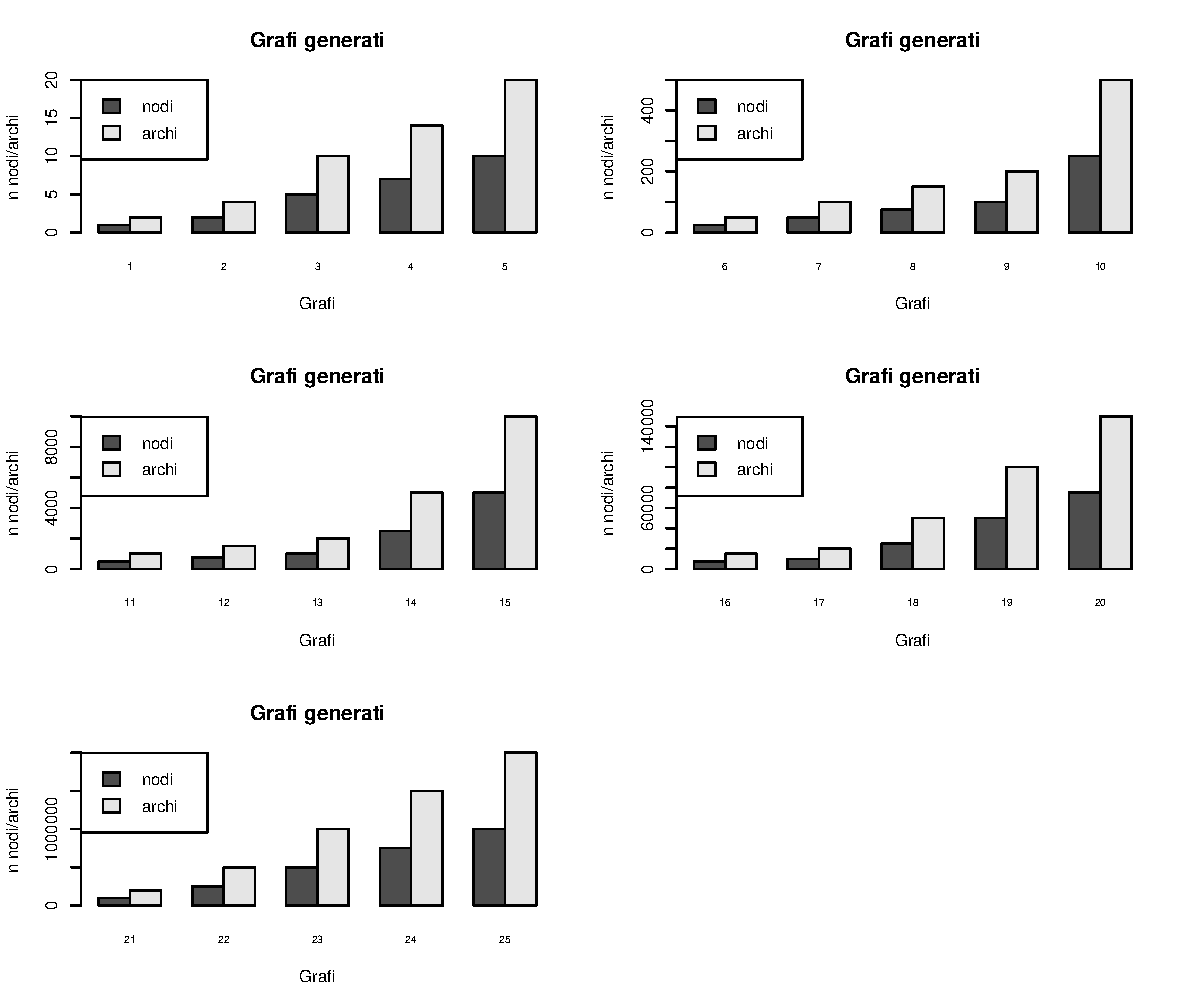
\includegraphics[scale=0.75]{benchmark_grafi}
\caption[Grafico a barre dei grafi generati]{Grafici a barre relativi i numeri di nodi e archi dei grafi generati.}
\end{figure}
\captionsetup{justification=justified, singlelinecheck=false}
Per il numero dei nodi dei grafi generati si sono prese in considerazione
le potenze di dieci generando, all'aumentare dell'esponente, grafi il cui
numero di nodi ripercorreva i fattori 1, 2.5, 5, 7.5 e 10.
Si sono creati quindi 25 grafi, raggiungendo la soglia
del milione di nodi, collegati tra loro da due milioni di archi.


\captionsetup{justification=centering, singlelinecheck=false}
\begin{figure}
\centering
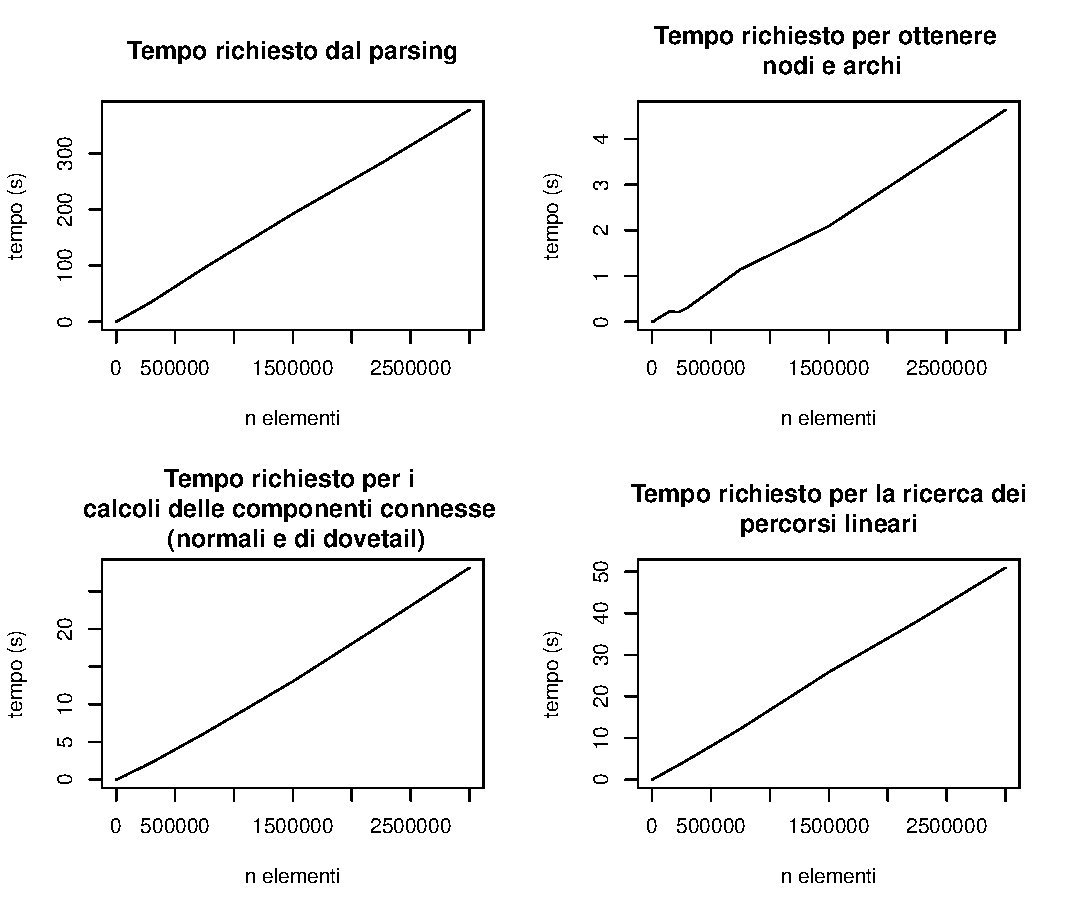
\includegraphics[scale=0.75]{benchmark_tempi}
\caption[Grafici dei tempi di calcolo delle operazioni su grafo]{Misurazioni dei tempi di calcolo.}
\label{fig:bench-timings}
\end{figure}
\captionsetup{justification=justified, singlelinecheck=false}
I tempi (figura \ref{fig:bench-timings}) indicano un andamento lineare
per tutte le operazioni eseguite. Il caso peggiore si ha nel caso
della funzione di ricerca delle sequenze di unitig, la quale
impiega un tempo doppio rispetto la ricerca delle componenti connesse.
I tempi per la lettura del file sono lineari e strettamente vincolati
dal tempo di accesso del supporto magnetico, si può pensare di ottenere
un risultato decisamente migliore usando un SSD, visto che
ha un tempo accesso più veloce.

\clearpage
\captionsetup{justification=centering, singlelinecheck=false}
\begin{figure}[h]
\centering
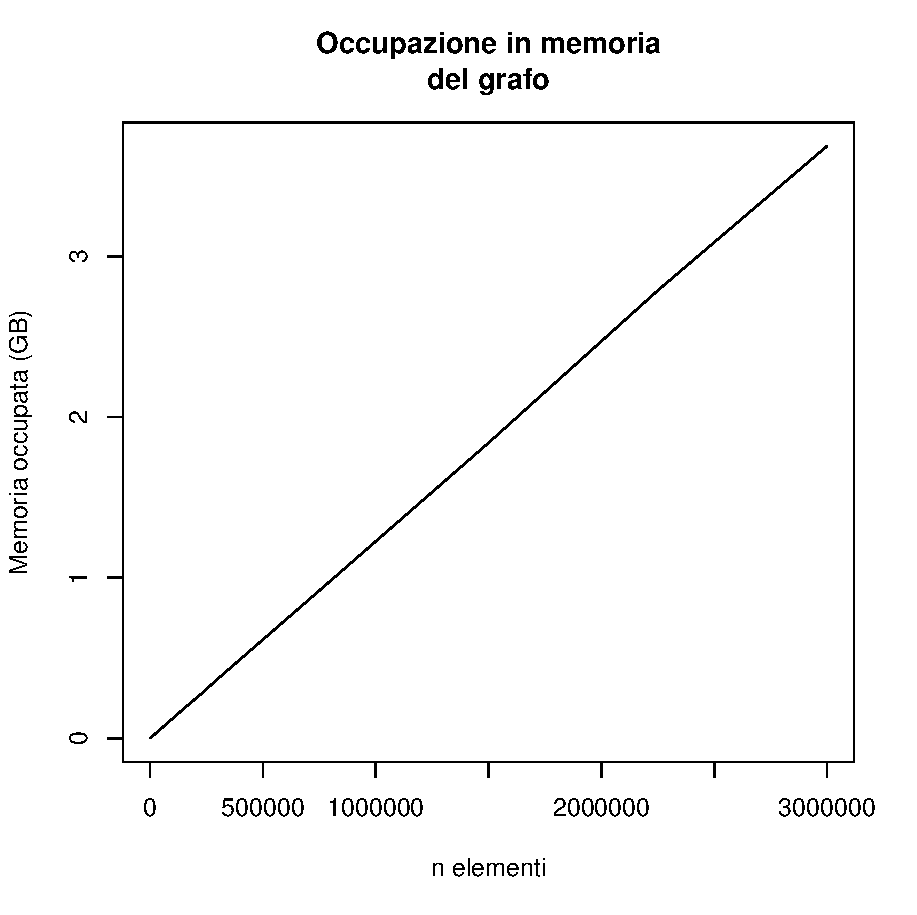
\includegraphics[scale=0.75]{benchmark_memoria}
\caption[Grafici della memoria occupata dal grafo]{Misurazione della memoria occupata dal grafo.}
\label{fig:graph-memory}
\end{figure}
\captionsetup{justification=justified, singlelinecheck=false}
L'uso della libreria NetworkX, come già accennato a pagina \pageref{sec:nx-why-limits},
comporta una grossa occupazione della memoria. I dati riportati nel grafico
in figura \ref{fig:graph-memory}
riguardano il peso del grafo GFA subito dopo la sua creazione da file, senza
prendere in considerazione la memoria di ``contesto'' necessaria per avviare
il processo Python e la libreria standard. In totale la memoria occupata
raggiungeva, nell'ultimo grafo, circa i \SI{4.2}{\giga\byte} raggiungendo
il limite di \SI{5.1}{\giga\byte} durante la ricerca dei percorsi lineari, operazione
che si è rivelata essere la più dispendiosa fra quelle misurate.

% Confronto Gfapy e PyGFA
\section{Confronto con Gfapy}
Nei seguenti grafici sono indicati i dati ottenuti eseguendo, con le librerie
Gfapy e \pygfa, le operazioni di parsing ed estrazione degli elementi del
grafo da un file gfa, estrazione dei dizionari contenenti le informazioni
del grafo e calcolo delle componenti connesse; mostrando
le differenze sia in termini di tempo di esecuzione (figura \ref{fig:comparison-times})
che di spazio occupato (figura \ref{fig:comparison-memory}).

Per ottenere questi dati sono stati generati grafi casuali fino ad un limite massimo di cinquemila nodi
e diecimila archi. Tale limite è dovuto a delle problematiche riscontrate con l'uso di Gfapy
per grafi con numero di elementi maggiore, oltre il quale
l'operazione di calcolo delle componenti connesse causa problemi dovuti
probabilmente alla natura ricorsiva del metodo implementativo in Python.
Come evidenziato dai grafici, il tempo di esecuzione relativo il parsing
è maggiore in Gfapy, mentre il tempo richiesto per accedere ai dizionari
contenenti gli elementi del grafo è pressoché costante in entrambe le librerie.
Per quanto riguarda il calcolo delle componenti connesse \pygfa \ è nettamente
più veloce. Infine dall'ultimo grafico è possibile notare come il
consumo di memoria richiesto è all'incirca il medesimo.

\captionsetup{justification=centering, singlelinecheck=false}
\begin{figure}[h]
\centering
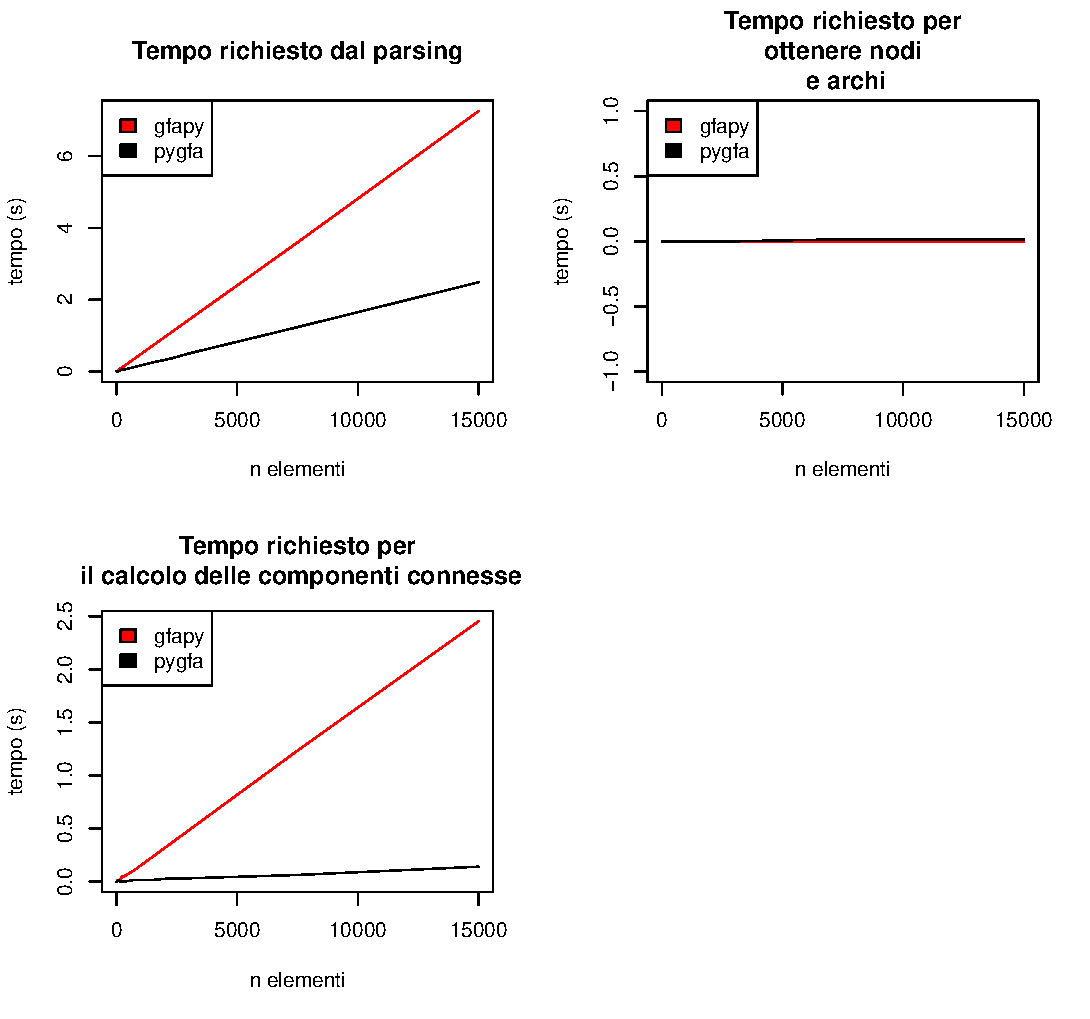
\includegraphics[scale=0.75]{comparison_times}
\caption[Grafici dei tempi di esecuzione di Gfapy e \pygfa]{Grafici dei tempi di esecuzione di Gfapy e \pygfa.}
\label{fig:comparison-times}
\end{figure}
\captionsetup{justification=justified, singlelinecheck=false}


\captionsetup{justification=centering, singlelinecheck=false}
\begin{figure}[h]
\centering
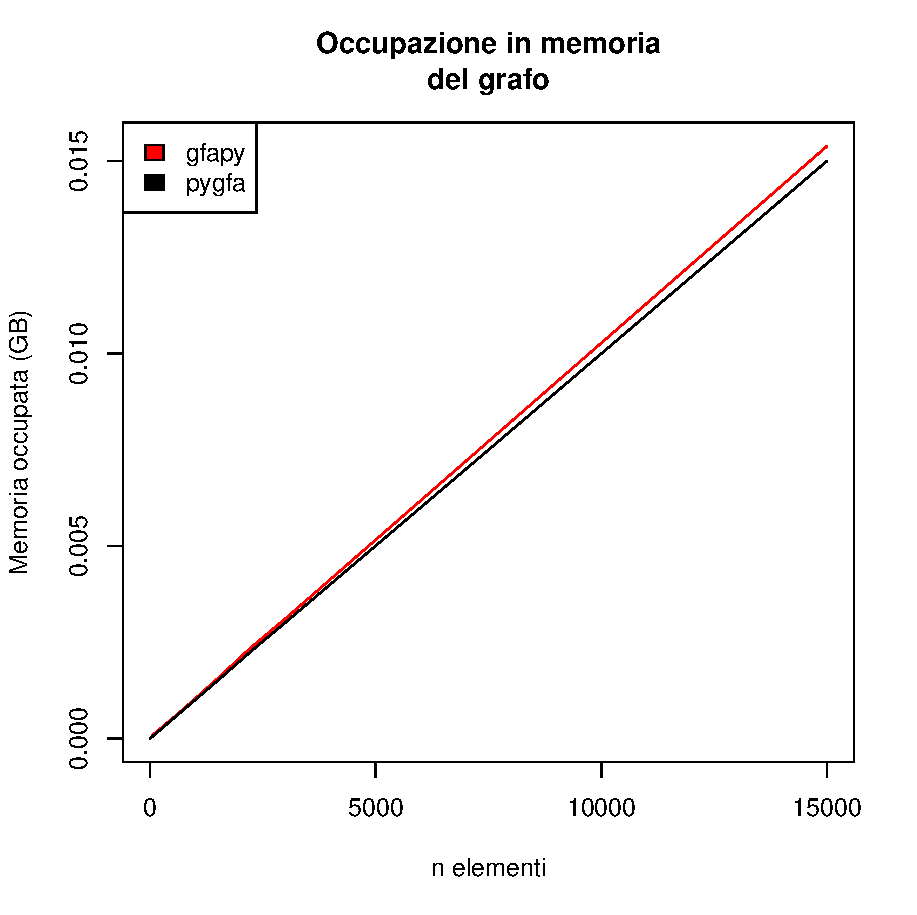
\includegraphics[scale=0.75]{comparison_memory}
\caption[Grafico della memoria usata da Gfapy e \pygfa]{Grafico della memoria usata da Gfapy e \pygfa.}
\label{fig:comparison-memory}
\end{figure}
\captionsetup{justification=justified, singlelinecheck=false}


\clearpage
\section{Conclusioni}
\pygfa \  ha gli stessi punti di forza e di debolezza di NetworkX:
le operazioni sono molto veloci, ma a costo della memoria occupata.
Nonostante ciò, la rapidità di sviluppo e l'ottima efficienza di questa libreria
rendono \pygfa \  un sistema performante molto facile da ampliare e modificare.
Messo a confronto con Gfapy, la libreria riesce ad eseguire alcune operazioni
in tempi decisamente migliori a parità di occupazione in memoria.


\chapter{Conclusioni}
In questo capitolo si riassumerà lo stato di sviluppo
di \pygfa, i problemi che ancora si riscontrano e di come
sarebbe possibile risolverli. Verranno infine presentate
le conclusioni personali sull'attività di stage presentando
ciò che si è imparato nel suo sviluppo.

\section{Prima release di \pygfa}
\begin{wrapfigure} {O} {0.4\linewidth}
	\begin{centering}	
		
\includegraphics[scale=0.5]{pygfa}
		\caption[Logo di \pygfa]{Logo di \pygfa.}
	\end{centering}
\end{wrapfigure}
\pygfa \   è alla sua prima release stabile, la copertura dei test
scritti si appresta sopra il 95\% e il numero di issue individuate
da PyLint si aggira sulle 280 ottenendo un voto dallo strumento
di 8,5/10.
Molta parte del lavoro è stata dedicata nel fornire un
ambiente che ricordasse NetworkX, sia per facilitare l'utilizzatore
sia per aiutare il futuro programmatore ad integrare nuovi moduli
della libreria nel sistema.
Il processo di sviluppo adottato ha aiutato a favorire i cambiamenti,
ad adottare strategie migliori man mano che le conoscenze aumentavano;
per questo la struttura della libreria risulta essere divisa in due metodologie
di integrazione delle funzioni di NetworkX. I primi algoritmi, riscritti
affinché venissero considerati solo archi di dovetail, sono delle
copie degli equivalenti offerti dalla libreria, modificati dei soli
nodi considerati durante le iterazioni; gli ultimi
sono stati invece pensati per essere riutilizzati da un qualsiasi iteratore
personalizzato, sfruttando la capacità del linguaggio di passare
funzioni (l'iteratore stesso) come parametri. Per questo motivo
\pygfa \  necessita di una fase di refactoring più profonda, che stabilisca
una struttura unica da rispettare.

L'astrazione dei dati rappresentati nel grafo è un altro problema
degno di nota, visto che in alcune situazioni genera ambiguità riguardo
le linee delle specifiche dalle quali le informazioni provengono.
Si può pensare di aggiungere un ulteriore campo agli elementi del grafo
specificando la provenienza dei dati, evitando così nelle fasi successive
di fare affidamento alle particolari configurazioni dei dati per risalire
alla linea di origine.

\section{Conoscenze acquisite}
Elencare le conoscenze che questo stage ha apportato
al mio curriculum informatico richiederebbe troppo spazio,
cercherò di riassumere le competenze acquisite che ritengo più
importanti. In primo luogo il processo di sviluppo usato: lo stage
mi ha permesso di lavorare con grande libertà per questo
un processo di sviluppo agile come extreme programming, 
che pone lo sviluppo al primo posto, mi ha senza dubbio
insegnato a gestire al meglio il tempo a disposizione e ad impostare
fin dal principio un progetto con delle fondamenta solide, ma allo stesso
tempo flessibili a futuri cambiamenti.

Imparare e usare Python durante lo sviluppo si è rivelato più
difficile del previsto; se da una parte permette una rapida prototipazione
ed un riscontro immediato delle funzionalità, dall'altra riuscire a
capire come strutturare un progetto corposo con un linguaggio
così flessibile richiede molta pratica. Nonostante questi
dettagli, imparare ad usare questo linguaggio e gli strumenti
di test di correttezza,  della qualità del codice e della documentazione
di progetto che gli sono di corredo ha accresciuto notevolmente
non solo la mia abilità nell'implementazione di un sistema nuovo, ma anche
l'approccio col quale se ne conduce lo sviluppo.

Concluderei questo capitolo e conseguentemente questa relazione
con ciò che questo stage mi ha permesso di apprezzare più di
ogni altra cosa: lo sviluppo di sistemi performanti in grado di
lavorare con una vasta mole di informazioni quali sono le informazioni
contenute dai grafi di assemblaggio. Nonostante \pygfa \  non
pone molta enfasi sulle prestazioni è stato possibile
esaminare i contesti e le situazioni nei quali un linguaggio di alto
livello come Python risulta meno indicato rispetto un linguaggio
di basso livello come il C e viceversa.


\printbibliography

%\listoftodos[TODO]

\end{document}